\subsection{Event Classification}\label{event_classification}


\begin{table*}[htbp!]
\caption{A summary of the number of events in this analysis for data, simulated signal, beam background, cosmic MC background, and beam-off data background (scaled to the data POT/triggers).  The final two columns show the efficiency and purity at different stages of the selection.\label{cutflowtab}}
\center
\begin{tabular}{l  c  c  c  c  c  c  c }
\hline
\hline
Selection stage & Data & Signal & Beam Bgd. & Cosmic MC Bgd. & Beam-Off Bgd. & Efficiency [\%] & Purity [\%]\\
\hline
% (0) No selection  & 734221 & 923.1 & 160637.4 & 623740.9 & - & - \\
(1) Pre-selection  & 70691 & 632.1 & 7629.6 & 7736.4 & 52838.4 & 69.4 & 0.9 \\
(2) Flash matching & 11135 & 417.5 & 2160.8 & 613.7 & 6642.8 & 45.1 & 4.2 \\
(3) Vertex reconstruction quality & 7704 & 329.9 & 1462.4 & 457.3 & 4708.4 & 36.0 & 4.7 \\
(4) Shower hit threshold & 1889 & 276.9 & 509.5 & 82.6 & 725.0 & 29.9 & 17.4 \\
(5) Electron-like shower & 453 & 139.5 & 105.5 & 15.6 & 156.4 & 15.0 & 33.5 \\
(6) Final selection & 214 & 83.8 & 41.5 & 9.3 & 82.3 & 9.1 & 38.6 \\
\hline
\hline
\end{tabular}
\label{cutflowtab}
\end{table*}


We define our signal as a CC $\nu_e$ or $\bar{\nu}_e$ interaction inside a fiducial volume in the MicroBooNE detector above an (anti-)neutrino energy threshold of 250 MeV. This analysis is optimised towards high energies and therefore we set this threshold to exclude a region where the efficiency begins to rapidly decrease. Our signal events are identified by the presence of an electron or positron shower in the final state, regardless of the presence of additional particles. Because MicroBooNE is not able to differentiate electrons from positrons and, therefore, $\nu_e$ versus $\bar{\nu}_e$, the resulting selection contains both particles. As a consequence, we calculate the final cross section for a combination of $\nu_e$ and $\bar{\nu}_e$.

A pure selection containing $\nu_e$ and $\bar{\nu}_e$ CC interactions requires the use of several variables to remove any cosmic rays and other beam-induced backgrounds which are mis-reconstructed as showers. Due to the variety of interaction modes and detector effects, some interactions may be incorrectly classified, merged with other particles, partially reconstructed, or entirely unreconstructed. In order to study the signal efficiency and various background contributions, we classify events in the MC simulation as follows:

\boldsymbol{$\nu_e$} \textbf{CC}: $\nu_e$ or $\bar{\nu}_e$ interactions with an energy above 250~MeV with the primary interaction vertex inside the fiducial volume. This is our signal classification.

\boldsymbol{$\nu_e$} \textbf{CC Out-FV}: $\nu_e$ or $\bar{\nu}_e$ CC interactions whose primary interaction vertex is reconstructed inside the fiducial volume, while the true simulated vertex is located outside the fiducial volume but inside the MicroBooNE cryostat. As such, these are classified as background.

\textbf{Cosmic}: MC cosmic ray particles generated by \texttt{CORSIKA}~\cite{corsika} which are selected as the neutrino candidate. %These cosmic rays are simulated concurrently with neutrino beam MC and accompany a neutrino interaction inside MicroBooNE.

\boldsymbol{$\nu_{\mu}$} \textbf{CC}: MC generated particles originating from $\nu_{\mu}$ or $\bar{\nu}_{\mu}$ CC interactions. This background category includes all interaction topologies.

\textbf{NC}: MC generated particles from a neutrino neutral current (NC) interaction, including all topologies except those including $\pi^{0}$ in the final state.

\textbf{NC} \boldsymbol{$\pi^{0}$}: MC generated particles for a NC interaction with one or multiple $\pi^{0}$ in the final state. We classify these separately as the photons originating from $\pi^{0}$ decays can closely mimic electron showers.

\textbf{Out-of-Cryostat}: This category contains neutrino candidates originating from simulated neutrino interactions within and outside the cryostat walls.

\textbf{Beam-Off Data}: Any neutrino candidates originating from the sample of data collected when the beam was off fall under this background category. It contains exclusively cosmogenically produced activity.

 \subsection{NuMI $\nu_{\lowercase{e}}$~+~$\bar{\nu}_{\lowercase{e}}$ Selection}\label{numi_nue_selection}

We combine information from the NuMI beam extraction with the scintillation light recorded by the MicroBooNE PMTs and with TPC pattern recognition techniques. The selection does not target a specific part of the electromagnetic (EM) shower phase space, neither in angle nor energy. In order to reject beam and cosmic ray interactions that could mimic our signal, we apply a selection divided into six stages. These are listed in Table~\ref{cutflowtab}, together with the number of signal and background events surviving each stage.


%This selection leverages information from the NuMI beamline and the scintillation properties of argon, coupled to the pattern recognition techniques of a TPC. We do not apply any direct cuts on the angle or the energy on the daughter particles from the neutrino interaction.


The selection efficiency shown in Table~\ref{cutflowtab} is defined as the number of selected $\nu_e + \bar{\nu}_e$ CC interactions with an energy above 250~MeV in the fiducial volume divided by the number of simulated $\nu_e + \bar{\nu}_e$ CC interactions with the same energy threshold in the fiducial volume before any selection is applied. The selection purity is defined as the number of selected $\nu_e + \bar{\nu}_e$ CC interactions in the fiducial volume with an energy above 250~MeV divided by the total number of selected neutrino candidates (signal and background). 


%%%%%%%
\subsubsection{Pre-selection}\label{section_fv_cut}

The goal of the first stage of the analysis is to identify events where a neutrino interaction happened inside a volume where they can be reliably reconstructed and has a flash coincident with the beam window. 

% This pre-selection requires (1) a reconstructed shower with a vertex within the fiducial volume and (2) a flash coincident with the beam window.
\texttt{Pandora} classifies each region of activity in the TPC as either a track or a shower. Our selection requires at least one reconstructed shower associated to the \texttt{Pandora} neutrino candidate. The \textit{leading shower} in the event is defined as the reconstructed shower object with the most charge deposition associated with it.

%We obtain the time during which the NuMI beam spill occurs and neutrinos are expected at MicroBooNE from the Fermilab Accelerator Division. We require flashes to be coincident with this NuMI beam spill window. 

The distribution of the reconstructed flash time is shown in Fig.~\ref{flash_time_data_everything} for data versus the stacked prediction of MC + NuMI beam-off data. The NuMI beam spill window occurs between 5.5 to 16.0~$\mu$s. We reject flashes reconstructed outside of this window. % of 5.5 to 16.0~$\mu$s are rejected. 
The shoulder of the flash distribution on either side of the beam window is due to the NuMI online trigger gate being slightly wider than the NuMI beam spill window. This region is dominated by the beam-off data and is well-modeled. The shape between 3 and 4.5~$\mu$s is driven by flashes induced by cosmic activity that happen before the NuMI online trigger which have late scintillation light arriving inside the NuMI online trigger window. Flashes between 17 and 19~$\mu$s are generated mainly by argon late-light scintillation from interactions that happened during the beam window. The abrupt change in the number of flashes for beam-on data around 12 to 15~$\mu$s is a result of the 4+6 slip-stacking configuration of the NuMI beam. The MC is generated uniformly across the beam window such that the integral is equivalent to the integral of the beam-on data. This has no impact on normalization of the prediction to beam-on data because we normalize to the total POT delivered.


\begin{figure}[htb]
% \center
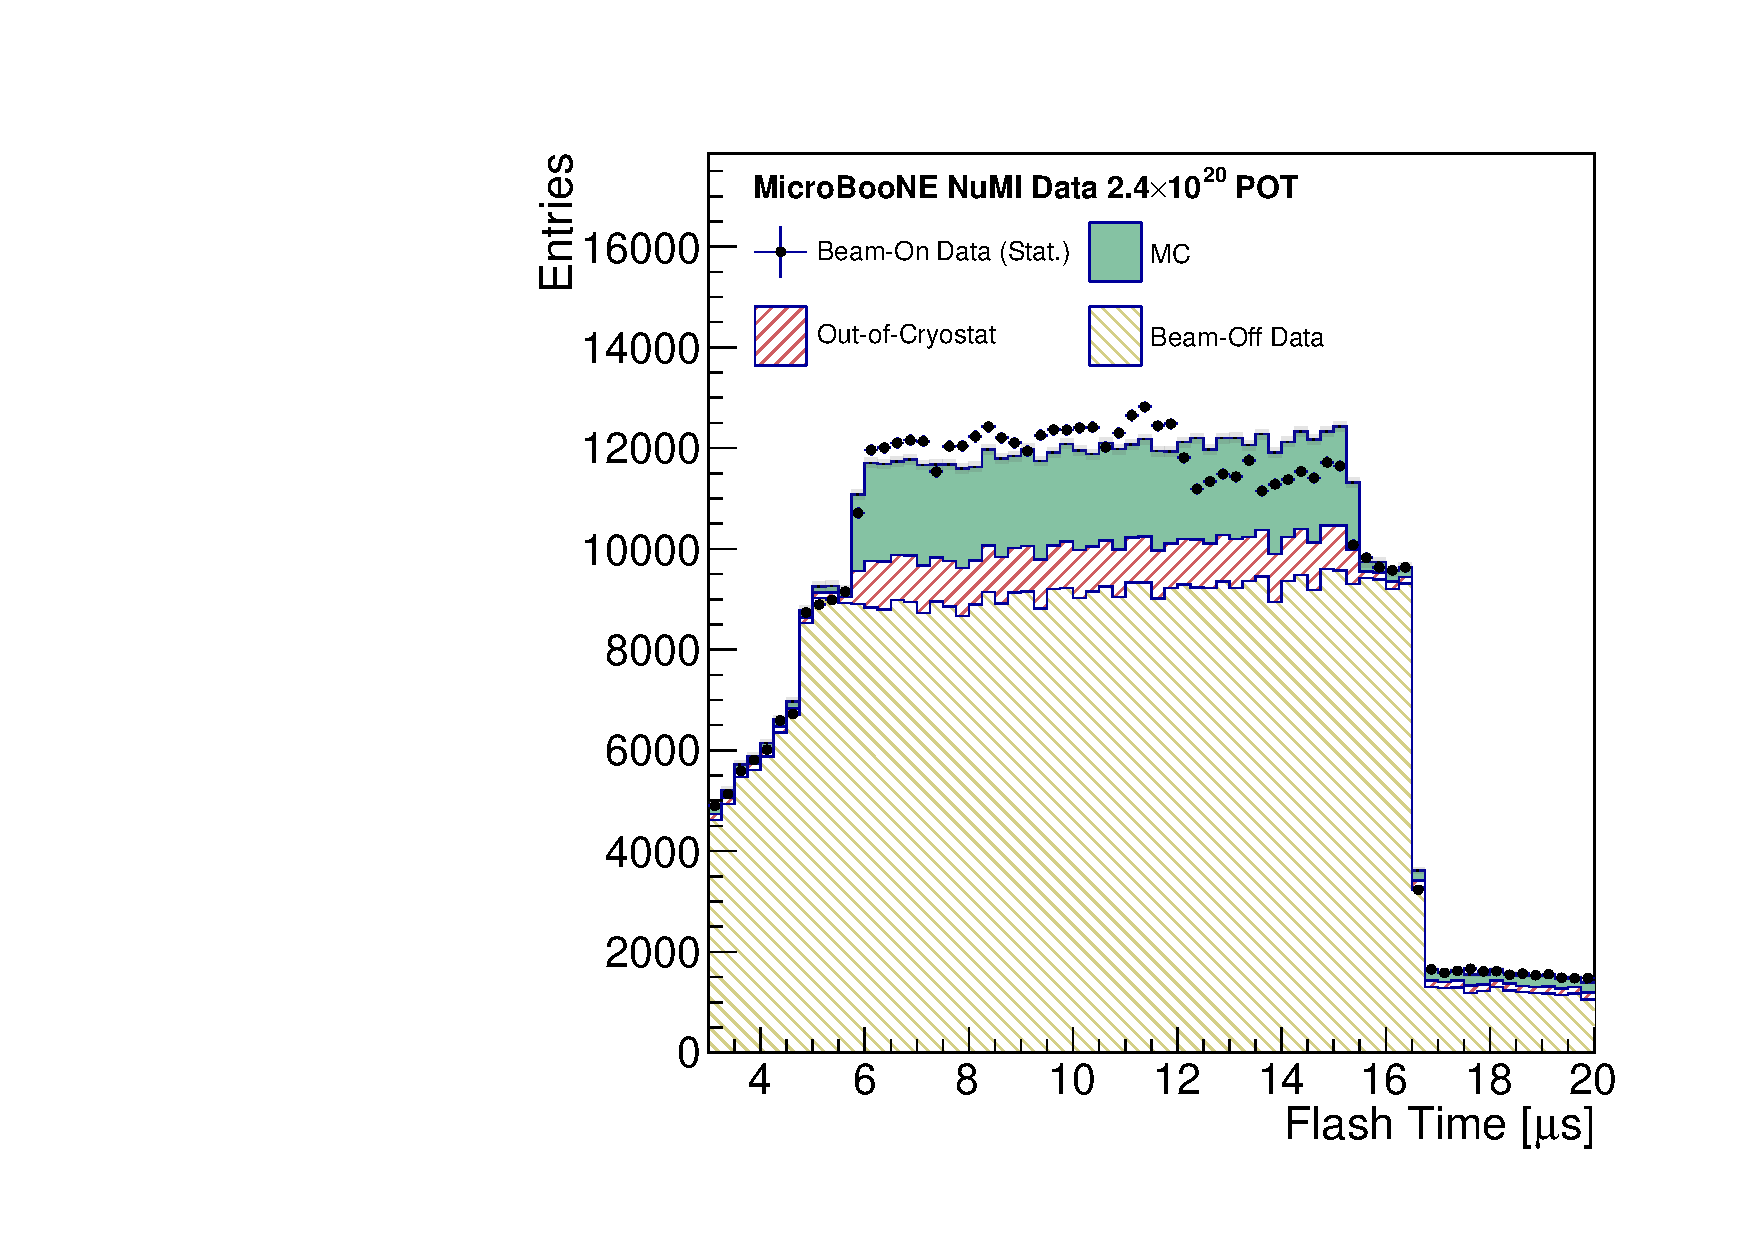
\includegraphics[width=\linewidth]{plots/flash_time_data_everything.pdf}
\caption{Beam-on data (points) compared to prediction (MC + NuMI beam-off data) for the reconstructed flash time before the selection is applied. The initial flash time corresponds to the start of the MicroBooNE detector readout window. The NuMI beam spill occurs between 5.5 and 16.0~$\mu$s, where the greatest number of flashes are observed.}
\label{flash_time_data_everything}
\end{figure}

A large fraction of cosmogenic activity is caused by low energy neutrons and photons which deposit less energy on average than neutrinos. We therefore reject neutrino candidates where the total light signal observed by the PMTs is less than 50~PE. This is a highly efficient method of removing a significant number ($\approx5\%$) cosmic ray backgrounds of which most are low energy.

%\floatbarrier
%%%%%%%%%%%%%%%%%%%%%%%%%%%%%%%%%%%%%%%%%%%%%%%%%%%%%%%%%%
%\subsubsection{Fiducial Volume}\label{section_fv_cut}

%The MicroBooNE cryostat extends beyond the instrumented portion of the TPC. 
% Particles interacting outside of the instrumented region can enter into the TPC active volume, resulting in interactions mimicking the signal. 
We define a fiducial volume in which we exclude 20~cm uniformly from all sides of the TPC, giving a total fiducial volume of $41.5$~m$^3$ (and a fiducial mass of 57.6~tonnes). Any neutrino interaction candidate with a reconstructed vertex outside of this volume is removed. This reduces the amount of selected out-of-cryostat and cosmic-ray interactions, and minimizes the impact of non-uniform electric field on the reconstructed tracks and showers near the cathode due to space charge accumulation~\cite{Abratenko_2020}.


%These pre-cuts are the starting point for the selection. % The selection efficiency is defined as the number of reconstructed $\nu_e$ CC events which pass the selection cuts over the number of true $\nu_e$ CC events in the fiducial volume as the denominator.
The efficiency for the pre-selection is 69.4\%. This large initial loss in efficiency is primarily driven by the shower reconstruction performance, where the electron from the $\nu_e$ CC interaction is either mis-reconstructed or not reconstructed at all. 
%$\epsilon = 3899 / 7103 = 54.89\%$
%The efficiency of the selection throughout this chapter is calculated using the number of reconstructed $\nu_e$ CC events which pass the selection cuts as the numerator and the number of true $\nu_e$ CC events in the fiducial volume as the denominator. The starting efficiency for the selection becomes $\epsilon = 3899 / 7103 = 54.89\%$. This large initial loss in efficiency is primarily driven by the shower reconstruction performance, where the electron in the $\nu_e$ CC interaction is often reconstructed either as a track or not at all. Recovering these interactions would likely require considerable work to do correctly and could be a clear area for improvement either at reconstruction or selection level.
%comment on if this is improved in MCC9
%The selection purity is defined here as the number of selected signal events divided by the total number of selected neutrino candidates, normalised to the POT of the On-Beam data. 
At this stage, the purity is 0.9\%, as the selection is dominated by the cosmic ray background.

\subsubsection{Flash Matching}
A powerful method to reject cosmic ray backgrounds is to combine the TPC and light information. This is known as ``flash matching''.
In this analysis we calculate the distance from the position of the largest flash (i.e. the flash with the most PE) occurring inside of the beam window to the reconstructed \texttt{Pandora} vertices in 2D ($yz$ plane). We assume that the largest flash in the beam window was produced by the neutrino interaction. The distance, ${\Delta Y\!Z}$, is constructed as:

\begin{equation}
\Delta Y\!Z = \sqrt{(z_{\text{flash}} - z_{\text{tpc}})^{2} + (y_{\text{flash}} - y_{\text{tpc}})^{2}}~,
\end{equation}

\noindent where $z_{\text{flash}}$ and $y_{\text{flash}}$ are the reconstructed center of the largest flash and $z_{\text{tpc}}$ and $y_{\text{tpc}}$ are the reconstructed neutrino candidate vertex coordinates. 

Compared to neutrino interactions, cosmic-induced backgrounds (beam-off and \texttt{CORSIKA} MC) tend to have larger match distances when compared with the largest optical flash registered during the beam window. We select events using the 2D match distance taking into account the relative positions of the flash and the TPC interaction vertices in the $z$ coordinate. Since the neutrino interactions are usually forward going, the flash center should be downstream of the neutrino interaction. This motivates a tighter selection if the reconstructed TPC vertex is downstream of the flash position:

\begin{equation}
\begin{split}
z_{\text{tpc}} > z_{\text{flash}} \rightarrow \Delta Y\!Z < 60~\textrm{cm}~,\\
z_{\text{tpc}} < z_{\text{flash}} \rightarrow \Delta Y\!Z < 80~\textrm{cm}~.
\end{split}
\end{equation}

%%%%%%%%%%%%%%%%%%%%%%%%%%%%%%%%%%%%%%%%%%%%%%%%%%%%%%%%%%
\subsubsection{Vertex Reconstruction Quality}

To mitigate backgrounds resulting from mis-reconstruction or incorrect particle hierarchy associations, we examine the distance of showers and tracks from the vertex, which is a metric of reconstruction  quality. This also removes background events where the leading shower originates from a photon. For example, in NC~$\pi^0$ events, the $\pi^0$  decays to two photons which pair convert after travelling some distance resulting in both showers being displaced from the vertex.

%We remove neutrino candidates where the reconstructed neutrino interaction vertex is unrealistically far from the leading shower or track start position.  
 
%The following two cuts compare the distance between the positions of the interaction vertex and the start position of the leading track or shower. This removes neutrino candidates where the reconstructed neutrino interaction vertex is unrealistically far from the simulated track or shower vertex, typically resulting from incorrect particle hierarchy associations or particles being mis-reconstructed. 

%\subsubsection{Shower Vertex Distance}\label{section_shower_vertex_cut}

We remove any neutrino candidates where the leading shower is reconstructed with a start point further than 4~cm from the neutrino vertex. This requirement applies only to the leading shower to ensure an inclusive selection of $\nu_e$ CC topologies which produce showers distant from the neutrino interaction (e.g. $\nu_e$ CC $\pi^0$ production). If the neutrino candidate event includes reconstructed tracks, we additionally require that at least one track must start within 4~cm of the reconstructed neutrino vertex; this additional selection removes events with associated cosmic activity, while allowing for some mis-recontruction effects due to unresponsive wires. After applying these vertex quality variables, the purity increases to almost 5\%, see Table \ref{cutflowtab}.

%%%%%%%%%%%%%%%%%%%%%%%%%%%%%%%%%%%%%%%%%%%%%%%%%%%%%%%%%%
\subsubsection{Shower Hit Threshold}

\begin{figure}[htbp]%thisone
\center
% \includegraphics[width=0.48\textwidth]{plots/pre_hit_cut_total_hits_leading_shower_data.pdf}
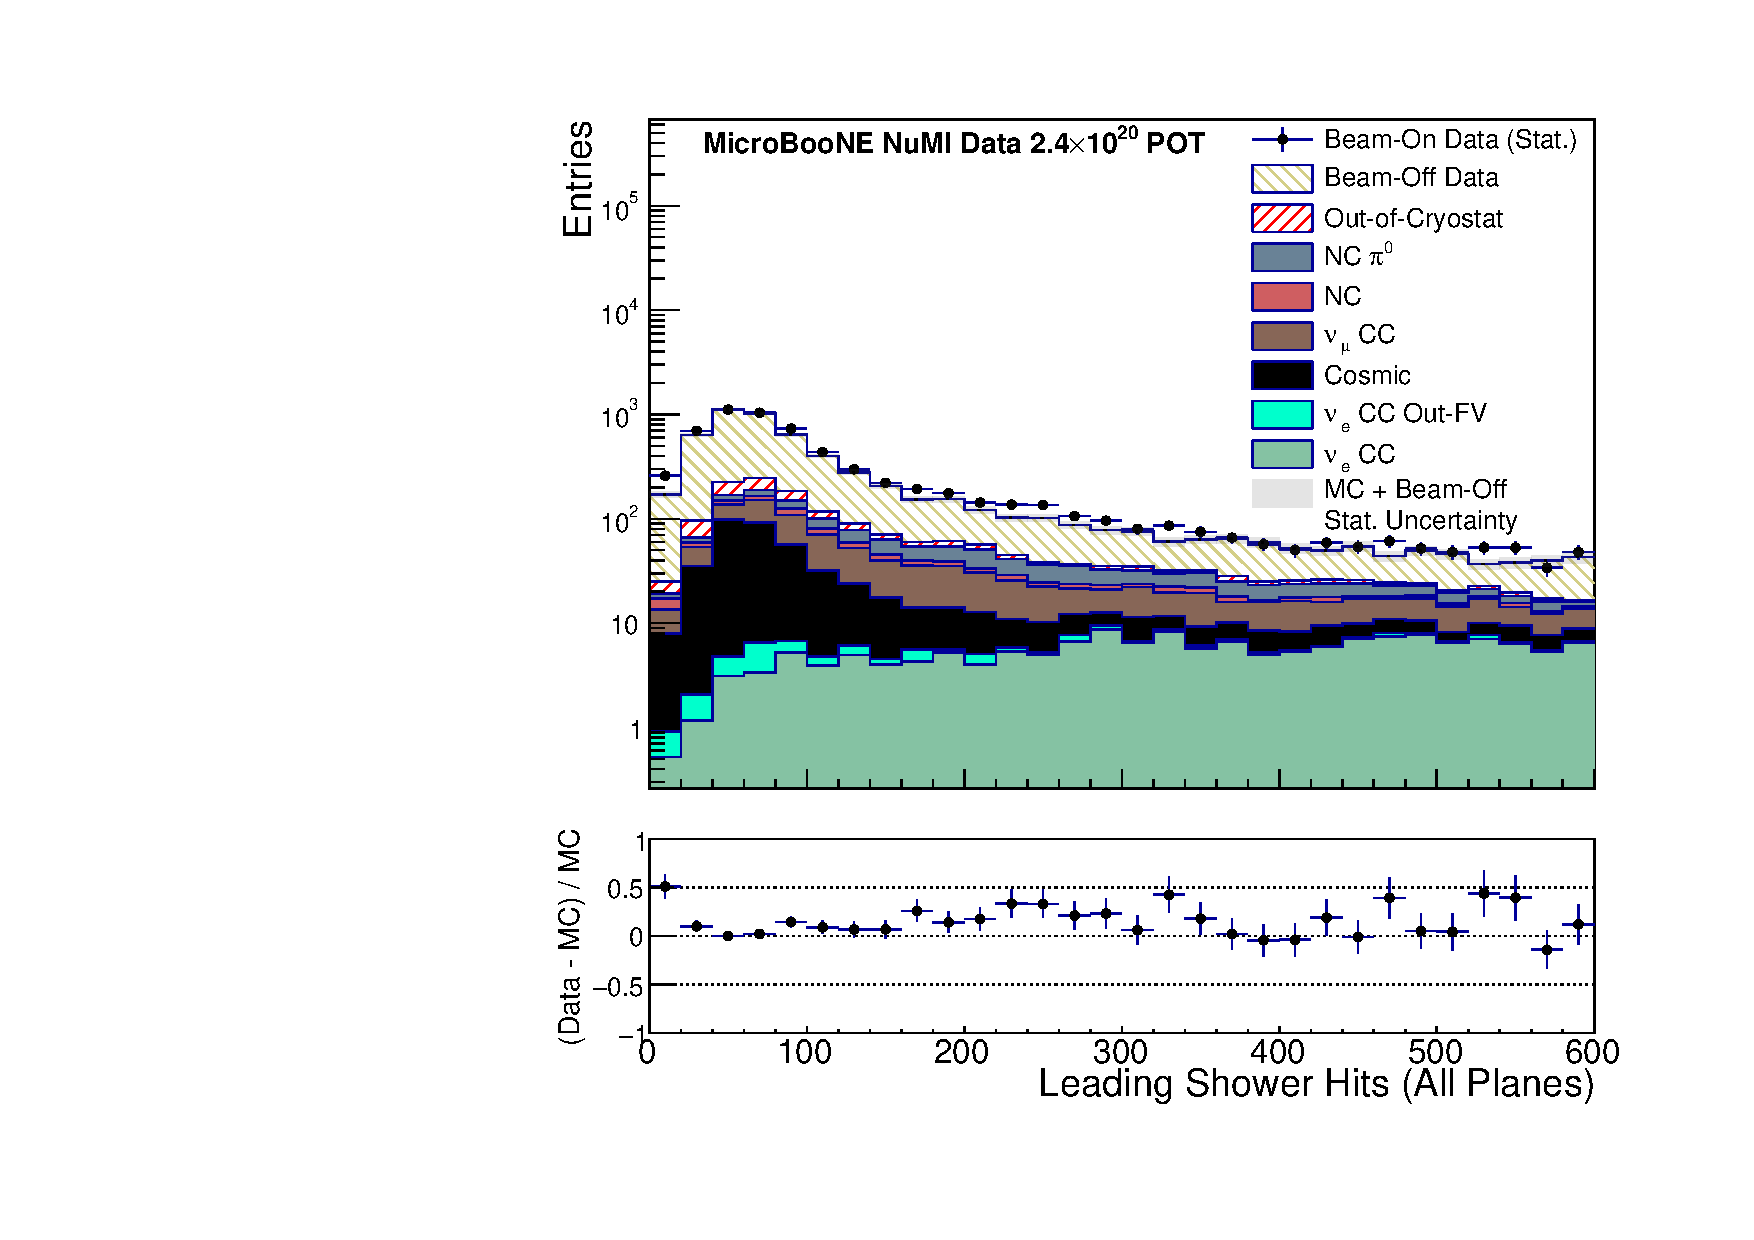
\includegraphics[width=\linewidth]{plots/pre_hit_cut_total_hits_leading_shower_data_logy.pdf}
\caption{Comparison of data (points) to the stacked prediction (MC + NuMI beam-off data) for the number of hits for the leading shower across all planes following the pre-selection, flash matching, and vertex reconstruction quality selection stages. }
\label{pre_hit_cut_total_hits_leading_shower_data}
\end{figure}

\begin{figure}[htbp]
\center
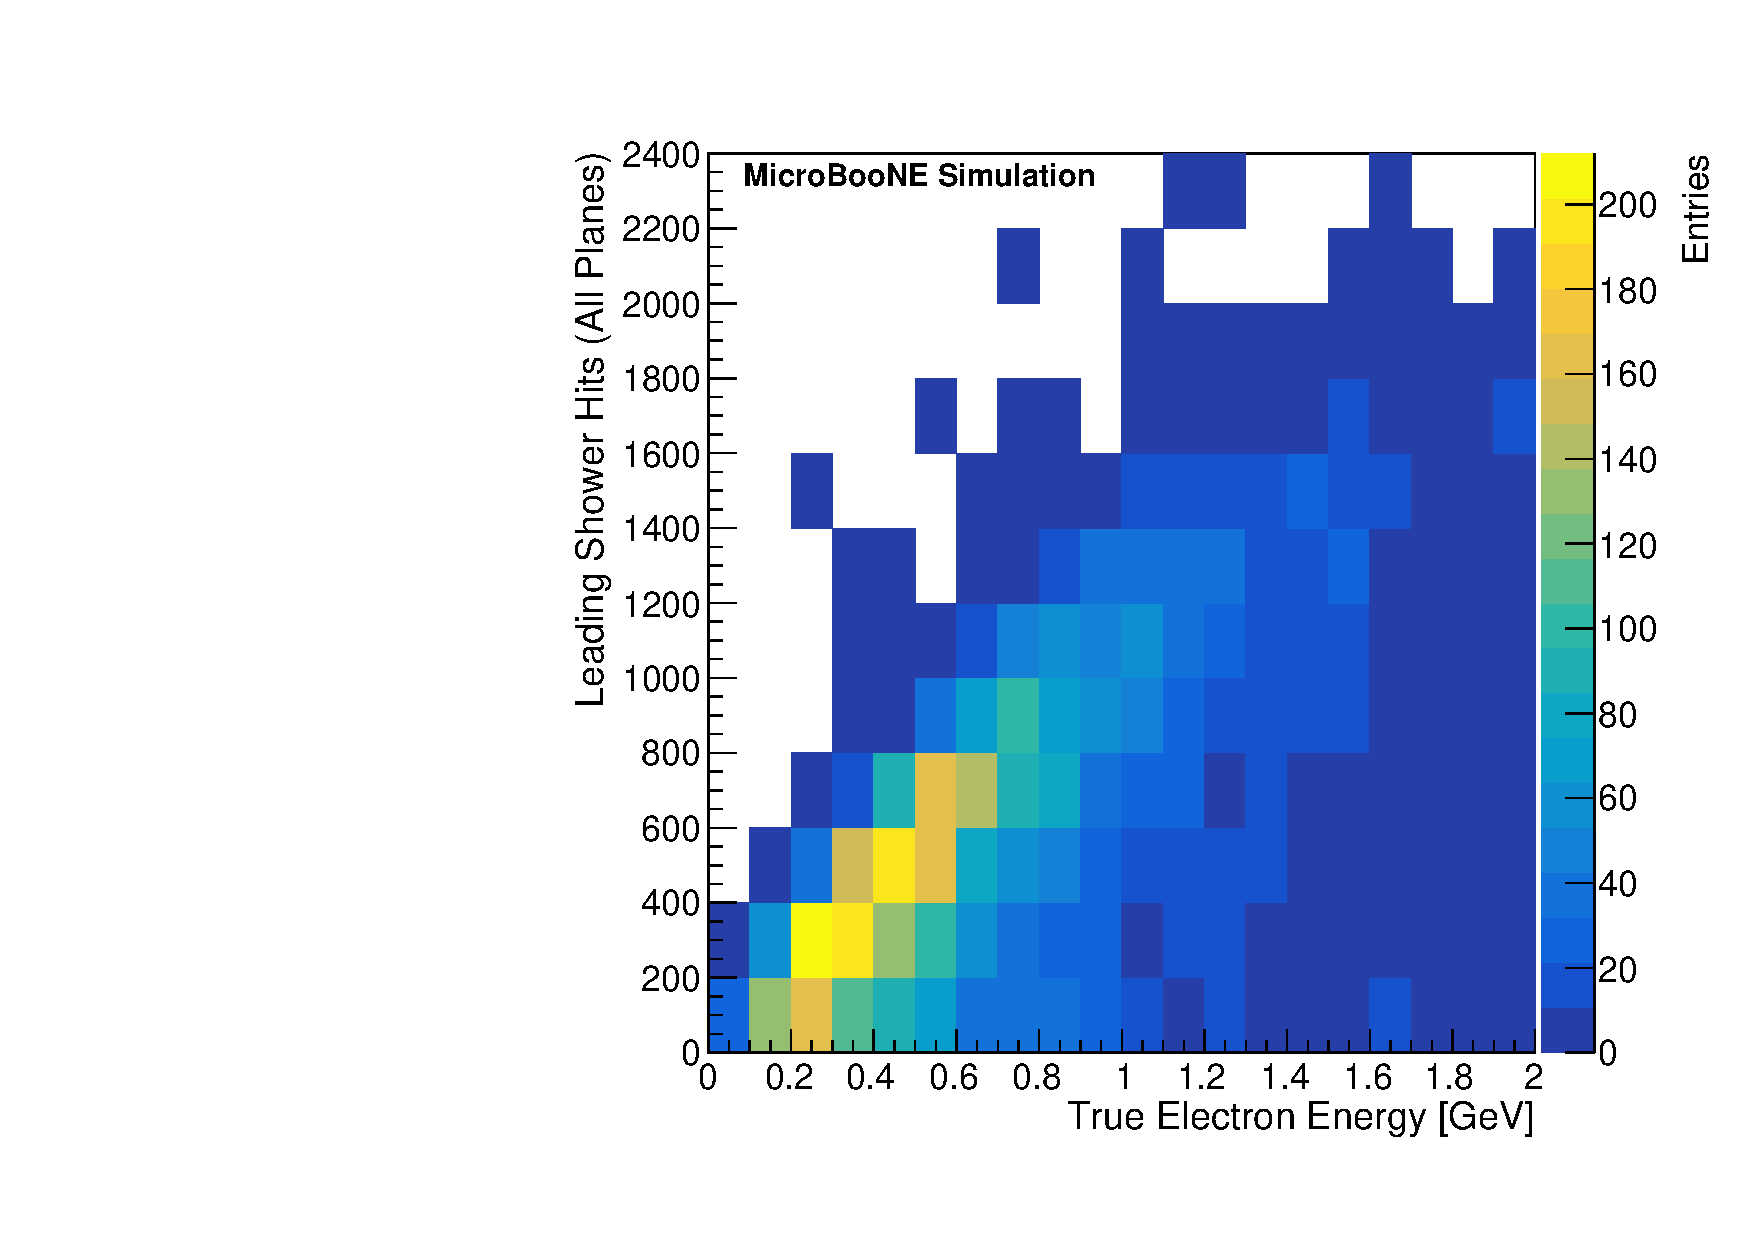
\includegraphics[width=\linewidth]{plots/shwr_hits_ele_eng.pdf}
% \includegraphics[width=0.48\textwidth]{plots_main/shwr_hits_ele_eng_zoom.pdf}
\caption{Number of hits in the leading shower (all planes) against true electron and positron energy for all simulated $\nu_e$ and $\bar{\nu}_e$ interactions.
}\label{shwr_hits_ele_eng}
\end{figure}


% As the selection requires at least one reconstructed shower, the leading shower is the key object to perform any validation of the neutrino interaction reconstruction quality.
The more hits that are associated to a shower, the easier it becomes to reconstruct its properties. Conversely, showers with very small numbers of hits are difficult to reconstruct precisely and are more likely to be affected by spurious charge depositions.
%Low energy showers and their properties (such as their initial dE/dx and direction) are difficult to reconstruct correctly due to their size. It is also far more likely for spurious charge depositions to be reconstructed as a low energy shower, whereas high energy showers with a substantial amount of TPC activity are a much cleaner topology.
We integrate the number of hits for the leading shower across the three wire planes; the resulting distribution is shown in Fig.~\ref{pre_hit_cut_total_hits_leading_shower_data}. The majority of the backgrounds cluster at values below 200 total hits in the leading shower, mainly due to mis-reconstructed muon tracks or the reconstruction splitting larger showers into sets of smaller showers. Requiring greater than 200 hits for the leading shower is effective at removing these mis-reconstructed showers, however, it impacts low energy neutrinos as well as background events. Figure~\ref{shwr_hits_ele_eng} shows the relationship between the simulated electron energy and the leading shower hits. While the total number of hits correlates with the energy of the shower, this correlation is non-trivial. We observe that this selection requirement removes events in a bin of electron energy just above 0.2~GeV, but a large population of such events are maintained.


%especially below 200 hits, where the relationship is non-linear. 
%While the total number of hits correlates with the energy of the shower, this correlation is not trivial. Figure~\ref{shwr_hits_ele_eng} shows the relationship between the simulated electron energy and the leading shower hits. Below 200 hits, the relationship between the electron energy and number of hits is not linear suggesting this selection requirement removes mis-reconstructed showers even if this impacts low energy neutrinos.

% maybe commenting on the fact that this bin (that we cut) is the least diagonal, showing that we’re cutting events that we can’t reconstruct well, even if it does mean we’re mostly cutting lower-energy events.

We also utilize the number of hits in the collection plane, which is typically the best-performing plane for reconstruction due to its high signal-to-noise ratio and is the plane used to calculate dE/dx at the start of the shower. Showers with few hits in this plane can lead to sizable uncertainties in the dE/dx measurement. Therefore, we require there to be at least 80 hits on the collection plane for the leading shower.


% \begin{figure}[htbp]%yes
% \center
% \includegraphics[width=\linewidth]{plots/post_cuts_collection_hits_leading_shower_data.pdf}
% \caption{Comparison of data (points) to the stacked prediction (MC + NuMI beam-off data) for the number of hits for the leading shower on the collection plane, following the requirement on the total hits. Background spectrum is clearly peaked around 100 hits, while most signal leading showers are at higher values.}\label{post_cuts_collection_hits_leading_shower_data}
% \end{figure}


\subsubsection{Electron-like shower}

The presence of an electron shower is the identifying characteristic for determining whether an event was induced by an electron neutrino interaction. To isolate such events, we employ the key feature of LArTPCs: the ability to distinguish photon-induced showers from electron-induced showers using a combination of calorimetric and topological information (i.e. the measurement of dE/dx and the distance between the shower and  interaction vertex). The initial dE/dx for showers induced by an electron correspond to the minimum ionizing particle (MIP) value. Showers induced from photons will instead register higher values of initial dE/dx corresponding to double MIP ionization. This is due to the electron-positron pair from photon pair production, which is the dominant interaction mode for photons at the energies of interest. Before the pair production occurs, a photon does not ionize the argon. This can lead to an identifiable gap from the vertex which becomes another clear signature of background EM-showers.

Where the previous selection variables address mainly the backgrounds from cosmic rays and shower quality, requirements on the leading shower opening angle and the shower dE/dx further remove tracks that are mis-reconstructed as showers (mostly beam-off data and $\nu_{\mu}$ CC interactions) and limit the contamination from photon-induced showers originating from NC $\pi^{0}$ and $\nu_{\mu}$ CC $\pi^{0}$ interactions. 

The shower opening angle, $\alpha_{\text{open}}$, is calculated using a principal component analysis (PCA) of the 3D hit positions of the reconstructed shower and is given by the equation:

\begin{equation}
    \alpha_{\text{open}} = \tan^{-1}\left(\frac{\sqrt{\textrm{PCA}_{\textrm{secondary}}}}{\sqrt{\textrm{PCA}_{\textrm{principal}}}}\right),
\end{equation}

\noindent where $\textrm{PCA}_{\textrm{principal}}$ and $\textrm{PCA}_{\textrm{secondary}}$ are the lengths of the principal and secondary eigenvectors. Figure~\ref{shower_open_angle_schematic} gives an intuitive view of this angle on a schematic of a reconstructed shower. The opening angle is a powerful discriminator for cases where tracks have been mis-reconstructed as showers. For example, cosmic rays with broken tracks near the neutrino interaction can be mis-reconstructed as the leading shower resulting in a large opening angle. We select neutrino candidates where $\alpha_{\text{open}}<15^{\circ}$. In order to remove neutrino candidates with a topology which is more track-like than shower-like, we require a minimum opening angle of $\alpha_{\text{open}}>3^{\circ}$. Figure~\ref{post_cuts_leading_shower_open_angle_data} shows the data versus MC prediction for shower opening angle before this requirement is made.

\begin{figure}[htbp]
\center
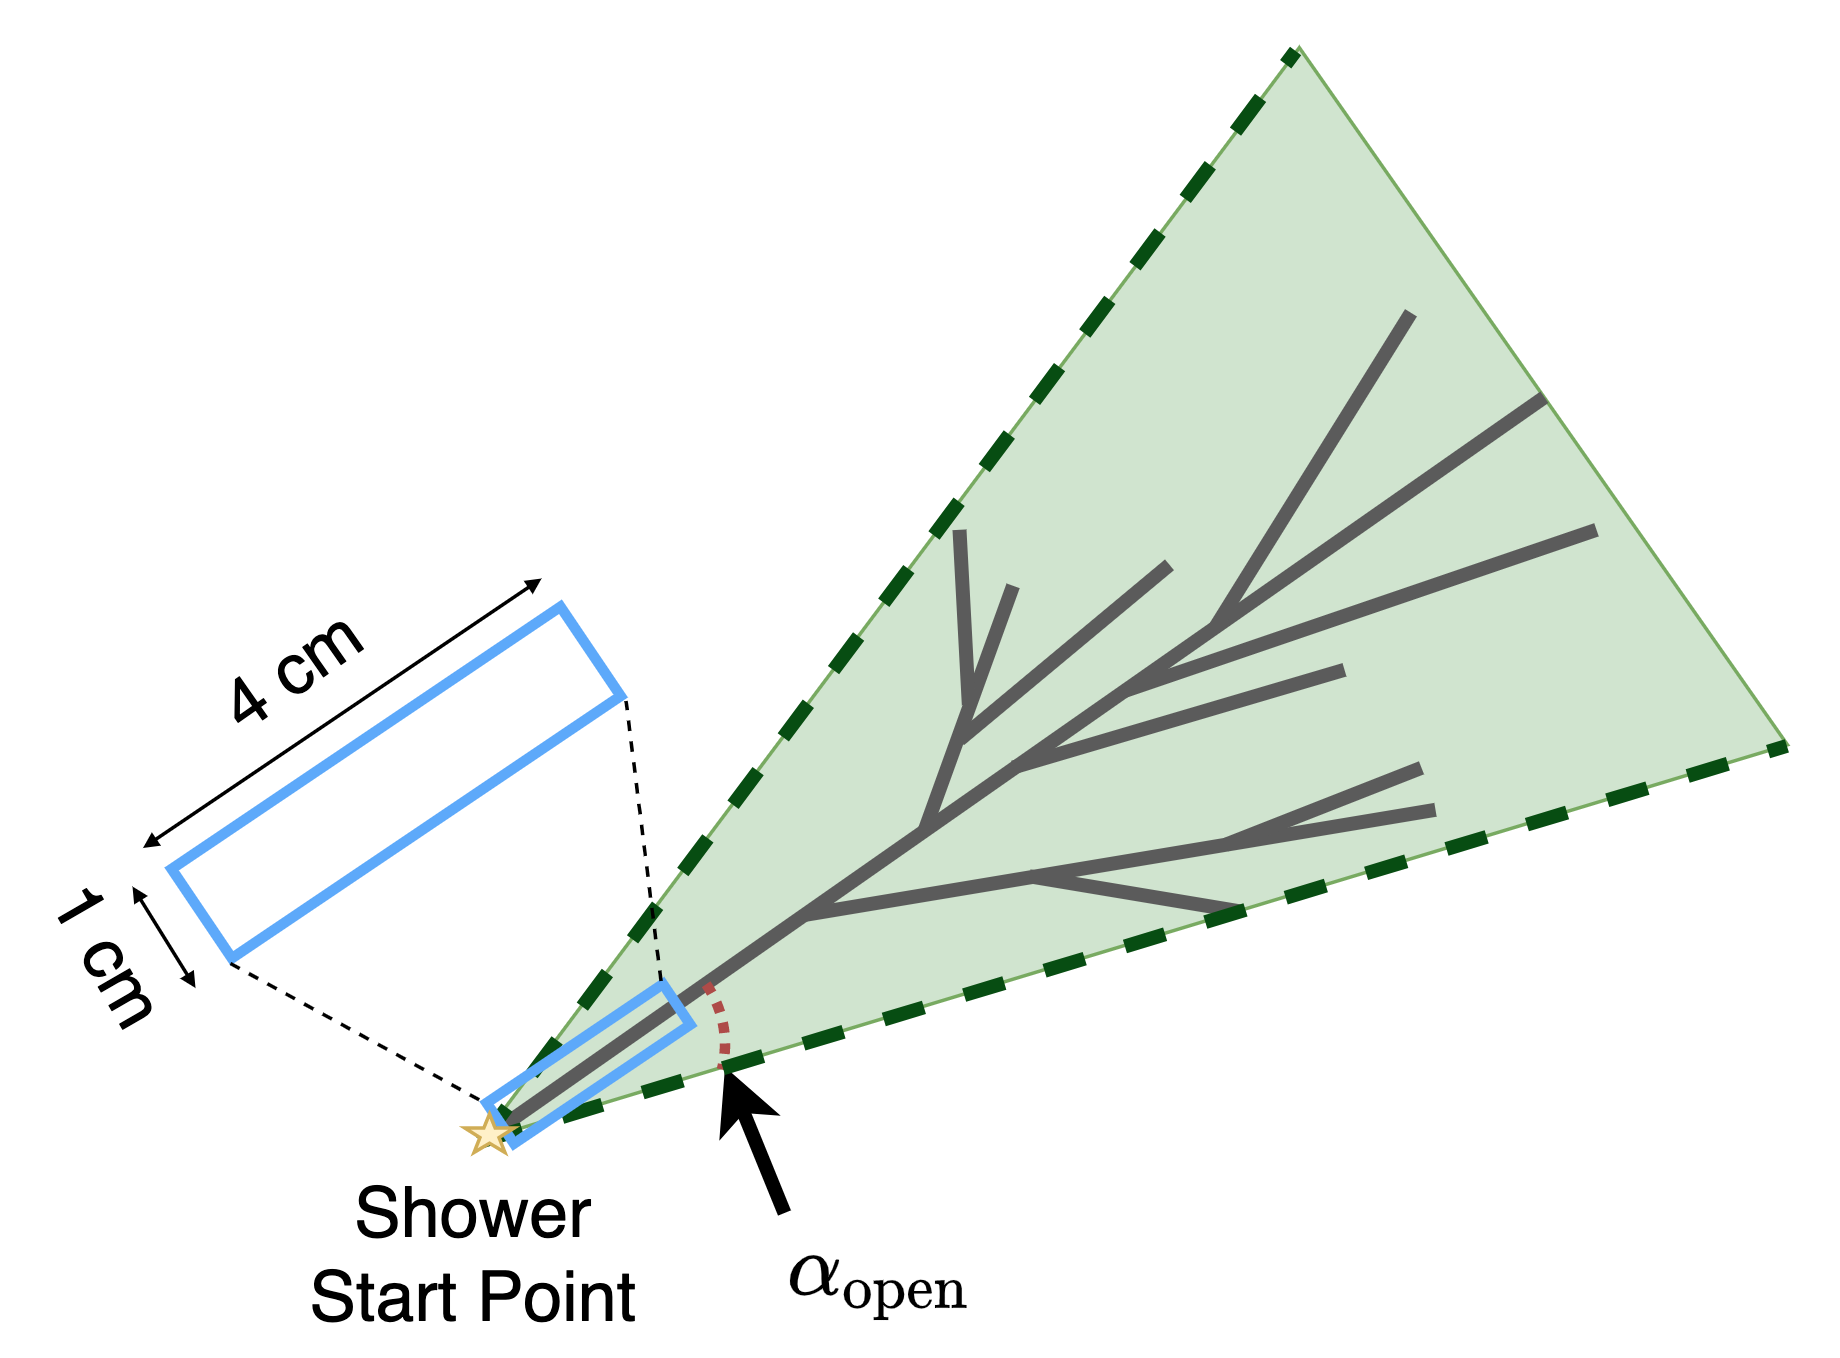
\includegraphics[width=0.35\textwidth]{plots/shower_open_angle_schematic.png}
\caption{Schematic showing the shower opening angle. The angle indicated by the dotted-red line shows the shower opening angle, $\alpha_{\text{open}}$. The median dE/dx calculation is performed using the charge deposition from the shower which falls within the box shown in blue.}
\label{shower_open_angle_schematic}
\end{figure}


 

% There is an overall shape agreement with an excess in data shifted towards higher values by a few degrees.

\begin{figure}[htbp]
\center
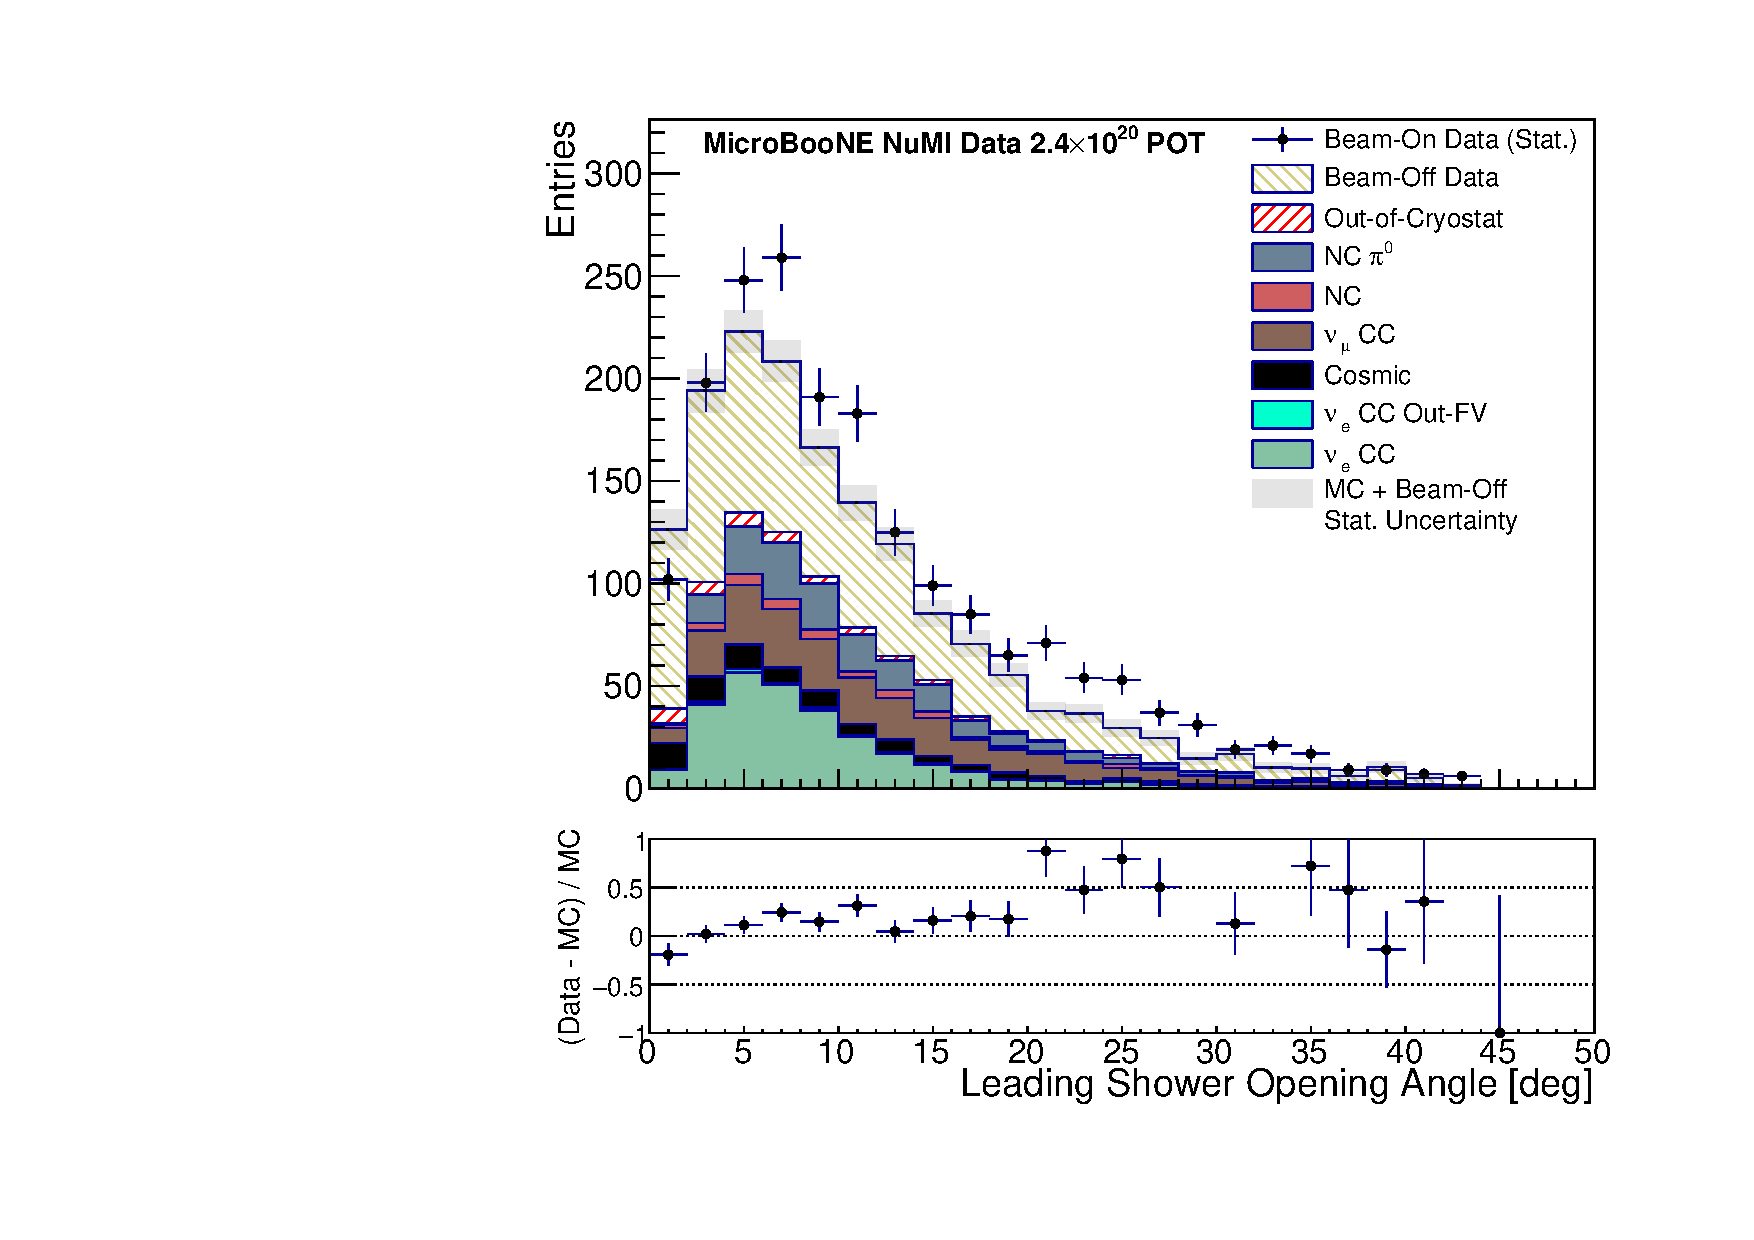
\includegraphics[width=\linewidth]{plots/post_cuts_leading_shower_open_angle_data.pdf}
\caption{Comparison of data (points) to the stacked prediction (MC + NuMI beam-off data) for the leading shower opening angle. Neutrino candidates pass the selection for leading showers between  3$^{\circ}$ and 15$^{\circ}$. }

% This plot is shown after all selection cuts from groups \textbf{(1)}, \textbf{(2)}, \textbf{(3)}, and \textbf{(4)} have been applied.}
\label{post_cuts_leading_shower_open_angle_data}
\end{figure}

%%\floatbarrier
%%%%%%%%%%%%%%%%%%%%%%%%%%%%%%%%%%%%%%%%%%%%%%%%%%%%%%%%%%
%\subsubsection{Shower dE/dx}\label{section_dedx_cut}

One of the most powerful features of LArTPC technology is that its entire volume is an active calorimeter. This means that the energy loss of a particle can be calculated along its trajectory, enabling the use of dE/dx for particle identification. Using the dE/dx in the first few centimeters of a shower is a powerful tool to distinguish electron-induced from photon-induced showers, as was demonstrated by ArgoNeuT \cite{Acciarri:2016sli}. Selecting the median dE/dx value as a truer representation of the shower's deposition profile rather than the arithmetic mean mitigates effects from single outlier hits which could result from Landau fluctuations as well as mis-configured electronics, detector effects, or mis-reconstruction.

The calculation of the median dE/dx is performed by constructing a $1\!\times\!4$~cm$^2$ box starting at the reconstructed shower start point, shown in Fig.~\ref{shower_open_angle_schematic} and calculating the dE/dx for the collection plane single charge deposits along the start of the shower. The charge deposits are converted to an energy using the Modified Box model~\cite{Acciarri:2013met}.

% Figure \ref{dedx_schematic} shows a very rough schematic of this technique.

% \begin{figure}[htbp]
% \center
% \includegraphics[width=0.6\textwidth]{plots/dedx_schematic.pdf}
% \caption{Rough schematic of the method used to calculate dQ/dx for reconstructed shower objects. The black lines represent a shower in the TPC. The blue box is the region used for calculating the dQ/dx and the red $x$ shows the reconstructed shower vertex. }\label{dedx_schematic}
% \end{figure}

Figure~\ref{post_cuts_dedx_cuts_data} shows the distribution of the calculated dE/dx on the collection plane wires for the leading shower using this method. The signal distribution peaks in the 2~MeV/cm region and large fractions of background lie to either side of the peak. Selecting those neutrino candidates whose dE/dx lies between 1.4~MeV/cm and 3~MeV/cm greatly increases the purity of the sample. As expected, the neutrino candidates containing photon-producing processes are centered around 4~MeV/cm. %Overall agreement between data and prediction is good.

\begin{figure}[htbp]
\center
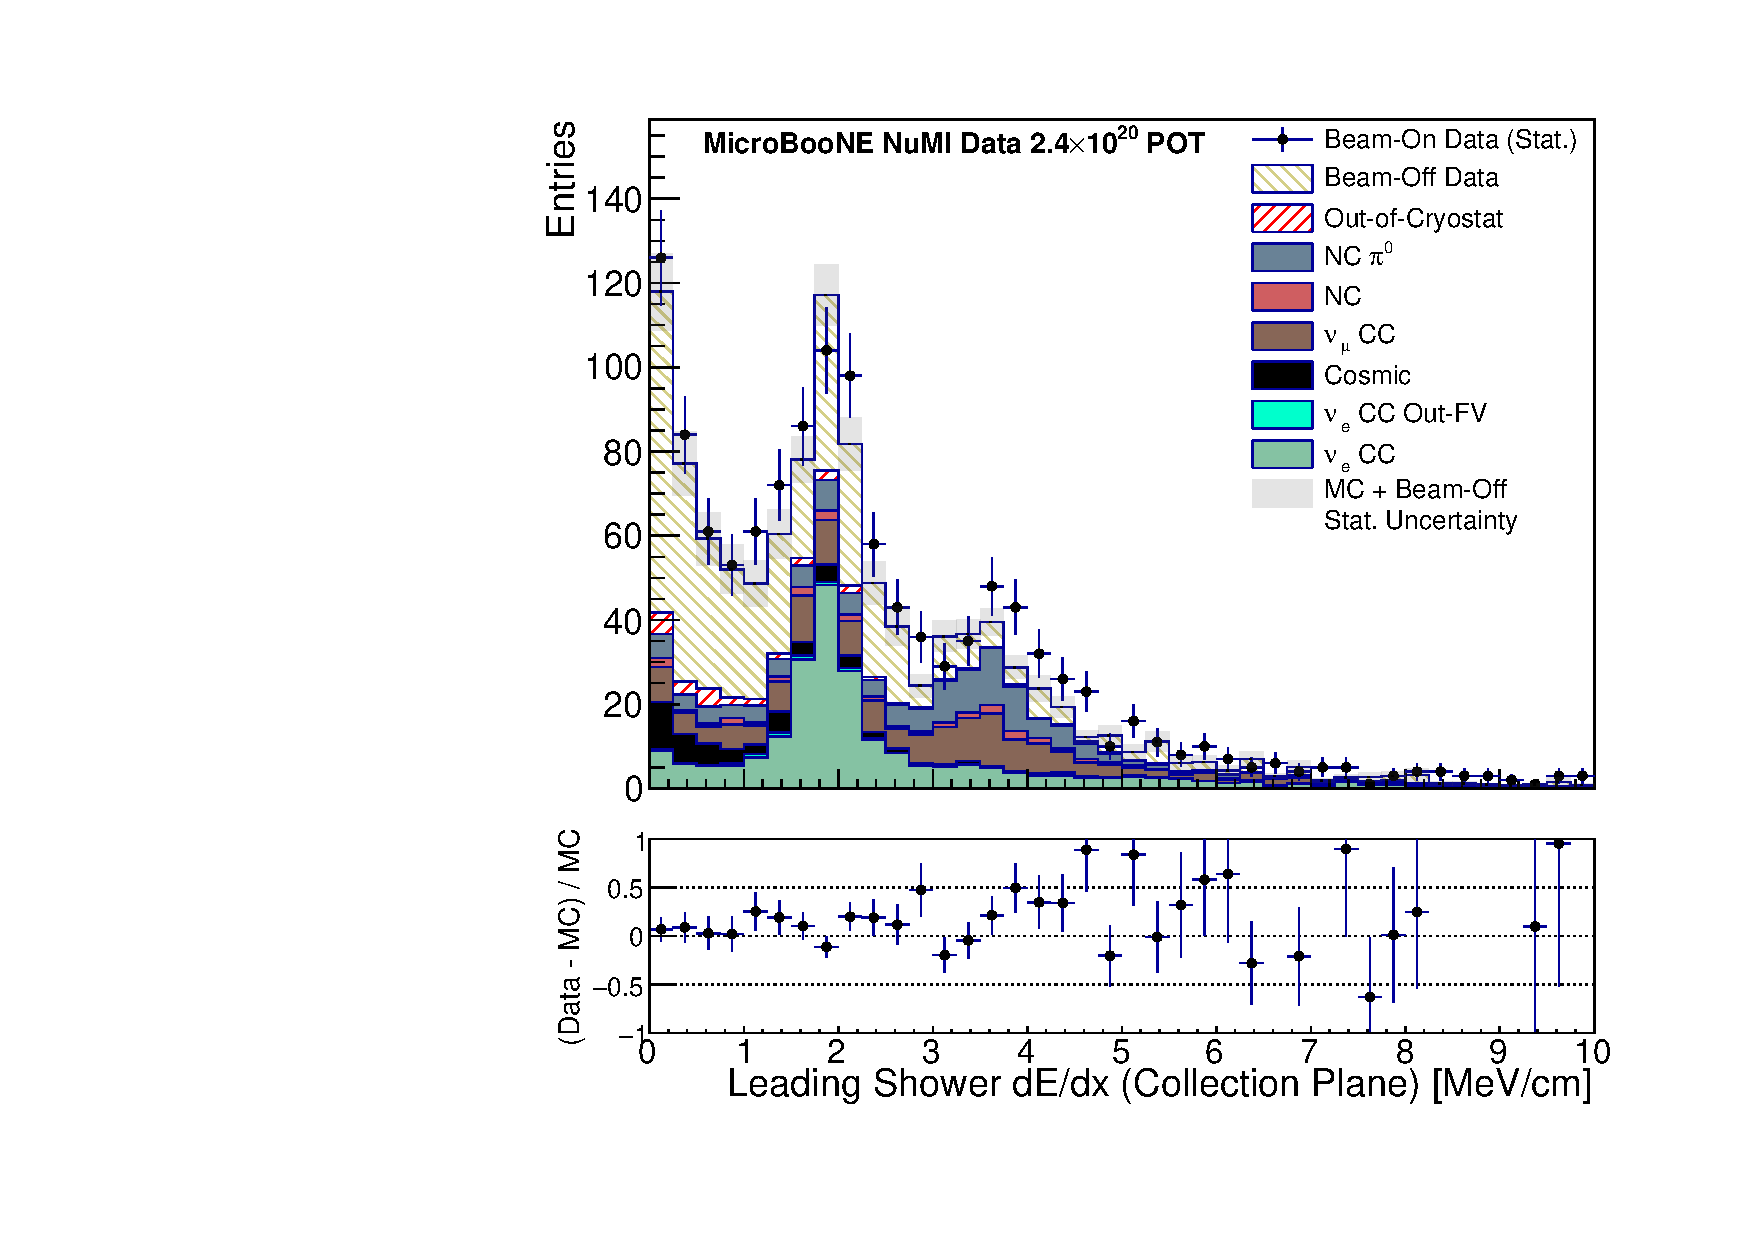
\includegraphics[width=\linewidth]{plots/post_cuts_dedx_cuts_data.pdf}
\caption{Comparison of data (points) to the stacked prediction (MC + NuMI beam-off data) for the leading shower dE/dx (calculated as described in text) distribution after the shower opening angle selection requirement. Signal interactions are peaked at 2~MeV/cm and beam-induced backgrounds are mostly peaked around 4~MeV/cm. A large number of background events are found between 0 and 2~MeV/cm.}\label{post_cuts_dedx_cuts_data}
\end{figure}

A notable feature in Fig.~\ref{post_cuts_dedx_cuts_data} is the large population of leading showers with a dE/dx of nearly 0~MeV/cm. This population is caused by tracks and showers that are nearly perpendicular to the beam direction ($60^{\circ}\!<\!\theta\!<\!120^{\circ}$) where it is challenging to measure dE/dx. In future analyses, this effect can be mitigated with the use of all three wire planes to measure dE/dx enabled by using methods such as 2D deconvolution as laid out in Refs.~\cite{signal_process_part1,signal_process_part2}.

Figure~\ref{post_cuts_dedx_theta_slice_1_data} shows the stacked data versus MC prediction where $\theta$ is between 0$^{\circ}$ and 60$^{\circ}$.  This slice of $\theta$ is the most populated region and has considerably higher purity than the rest of the phase space. As the dE/dx distribution at this angular slice includes showers running roughly perpendicular to the collection plane wires, a very small fraction of showers have an unphysically low dE/dx, which demonstrates the angular dependence of the dE/dx calculation in this analysis.


\begin{figure}[t]
\center
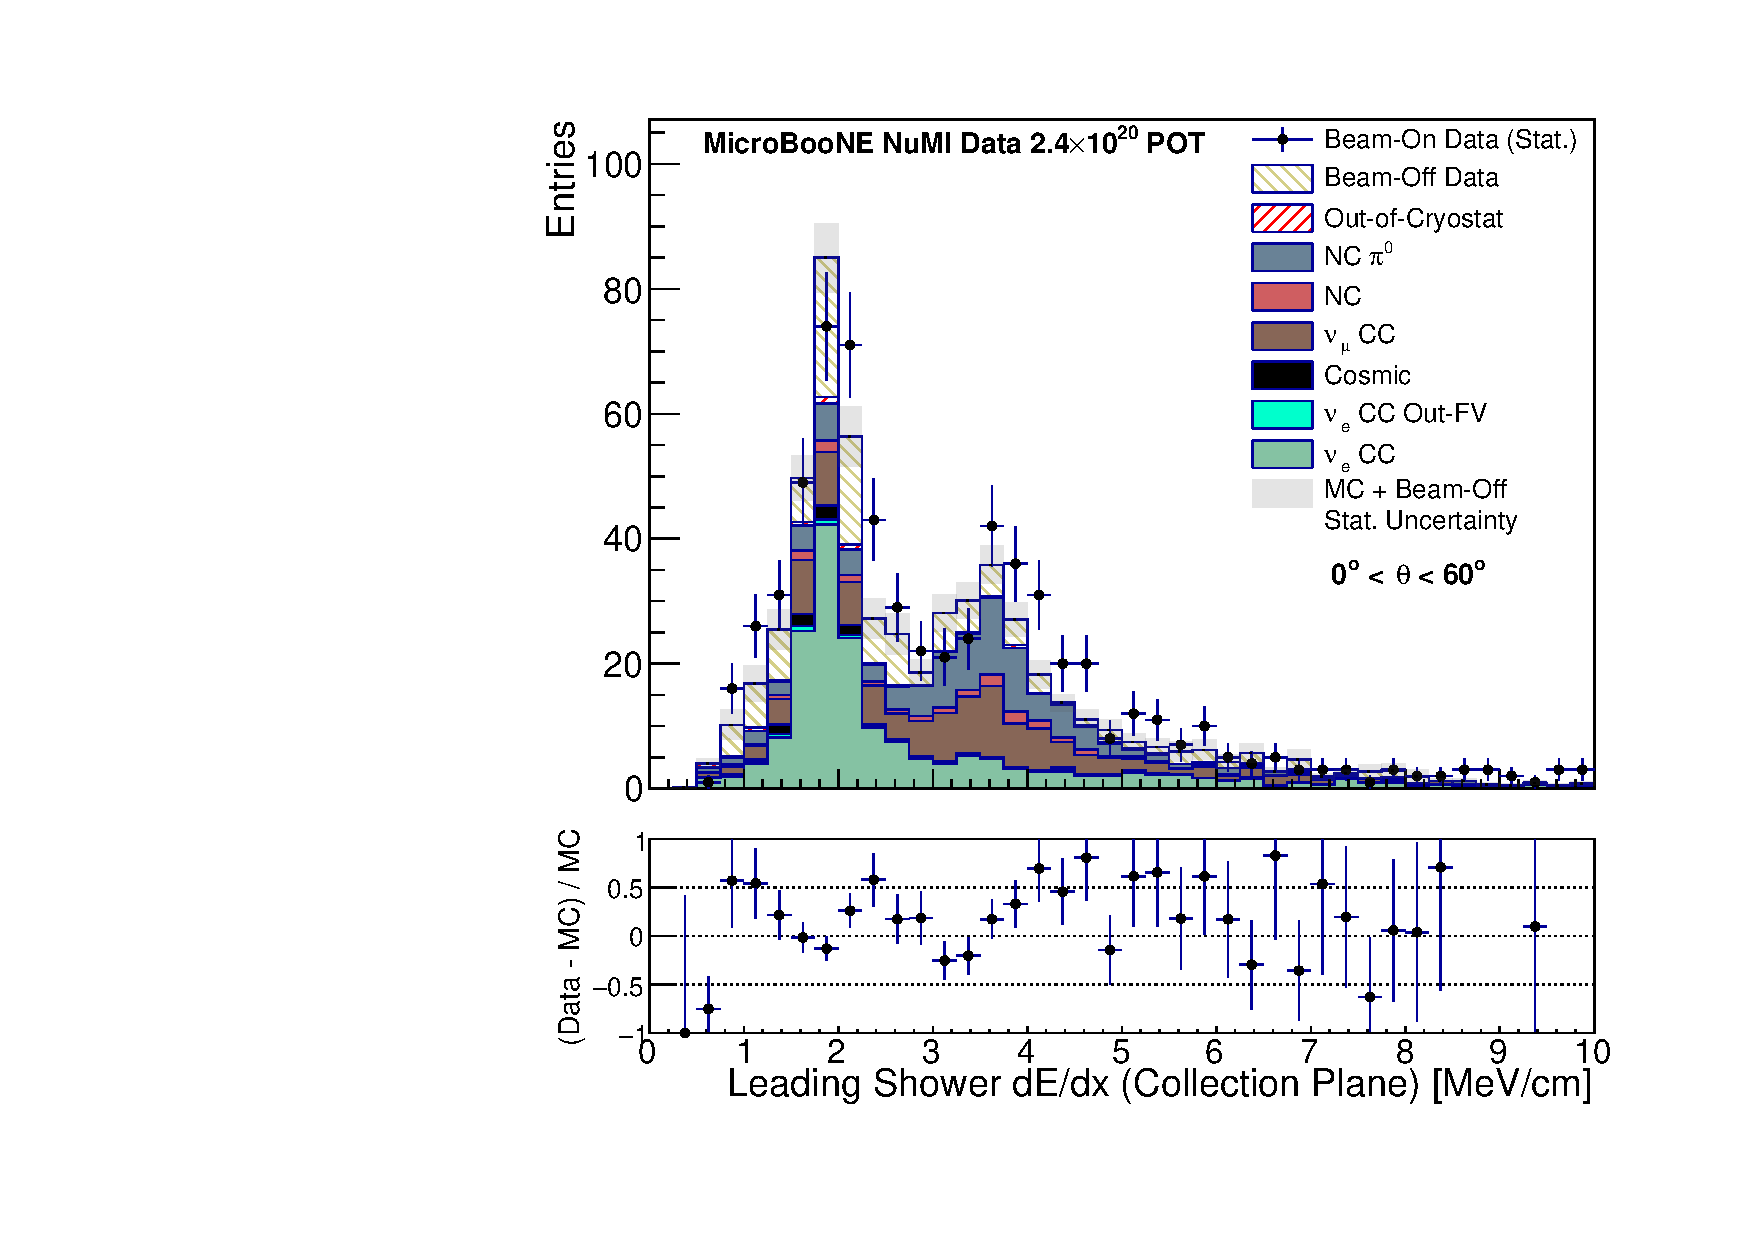
\includegraphics[width=\linewidth]{plots/post_cuts_dedx_theta_slice_1_data.pdf}
% \includegraphics[width=0.48\textwidth]{plots/post_cuts_dedx_theta_slice_1_zoom_data.pdf}
\caption{Comparison of data (points) to the stacked prediction (MC + NuMI beam-off data) for the leading shower dE/dx for a slice of $\theta$ between 0$^{\circ}$ and 60$^{\circ}$ after the shower opening angle selection requirement. In this angular range, the leading showers all have a well reconstructed dE/dx and the signal peak is well-defined.} %Plot on the right is an X-axis zoom into the signal region (0 to 4 MeV/cm).}
\label{post_cuts_dedx_theta_slice_1_data}
\end{figure}

For values of $\theta$ between 60$^{\circ}$ and 120$^{\circ}$, where the dE/dx is not well reconstructed, both the neutrino interactions and the considerable cosmic ray background are peaked at dE/dx values closer to 0 MeV/cm. In the range of $\theta$ between 120$^{\circ}$ and 180$^{\circ}$, we expect relatively few electron-neutrinos and a high contamination of cosmic rays. However, in this sample, the majority of the leading showers have well reconstructed dE/dx close to 2 MeV/cm.

%Given that the reconstructed leading shower direction can affect the calculation of the dE/dx, making a selection using the dE/dx has the potential to introduce an angular bias to the selection. In particular, removing neutrino candidates with dE/dx of below 1.4~MeV/cm from the selection causes a depletion of signal with leading showers with $\theta$ close to 90$^{\circ}$, however, this selection requirement is an extremely powerful tool for removing cosmic and beam-induced backgrounds which dominate at low dE/dx.
Given that the reconstructed leading shower direction can affect the calculation of dE/dx, using it may introduce an angular bias to the selection. %In particular, removing neutrino candidates with dE/dx of below 1.4~MeV/cm from the selection causes a depletion of signal with leading showers with $\theta$ close to 90$^{\circ}$, 
However, it is an extremely powerful tool for removing cosmic and beam-induced backgrounds which dominate at low dE/dx, as well as photon backgrounds at higher dE/dx values. Future analyses can mitigate the angular dependence of dE/dx by using three plane calorimetry.

This selection stage is successful in removing a large fraction of photon-induced shower backgrounds. Given the importance of removing these backgrounds in electron-neutrino analyses we explore the performance of photon-rejection variables further in Section~\ref{sec:dEdx}.



%This set of cuts is successful in removing not only photon-induced shower backgrounds but also cosmic and $\nu_{\mu}$ CC interactions. After this stage, the efficiency drops to 15.1\%, but the purity of the signal sample increases to 33.5\%. 

\subsubsection{Final Selection}

%\subsubsection{Secondary Shower Distance}


Mis-reconstruction of the neutrino candidate can lead to associating physically uncorrelated showers with the interaction. To remove these cases, we require the distance between the sub-leading showers and the neutrino candidate vertex to be less than 22 cm. The scope of this selection requirement is to mitigate mis-reconstructed showers while retaining a sizable fraction of $\nu_e$ CC $\pi^{0}$ interactions ( 44\%  relative to the previous selection stage).

% Because the conversion length of the gammas from a $\pi^0$ in argon is 11~cm, this selection requirement does not impact the majority of well-reconstructed signal neutrino candidates containing a $\pi^0$.

\begin{figure}[htbp]
\center
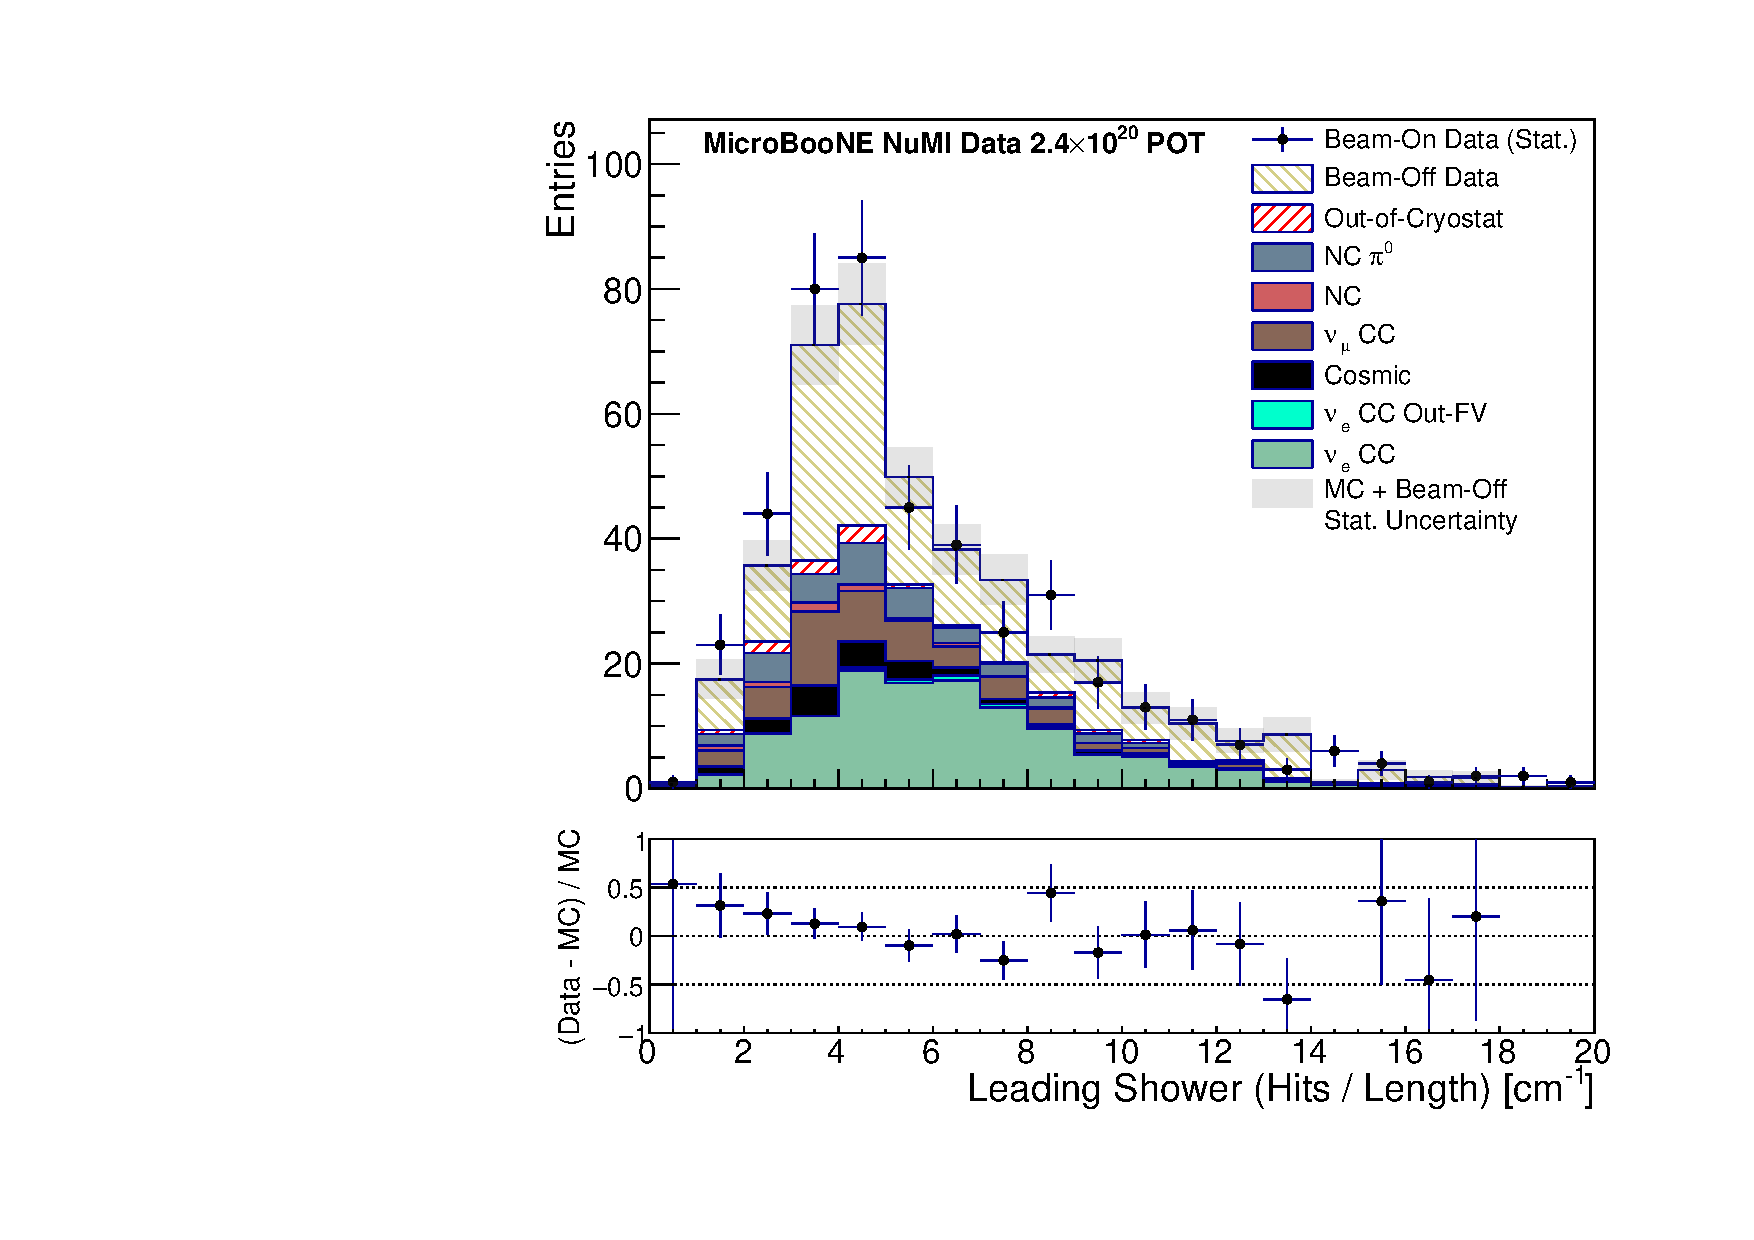
\includegraphics[width=\linewidth]{plots/post_hit_length_ratio_data.pdf}
\caption{Comparison of data (points) to the stacked prediction (MC + NuMI beam-off data) for the leading shower hit density variable after the selection requirement on the sub-leading shower distance to the vertex. The threshold is placed at 3~hits~per~cm where all neutrino candidates that have a leading shower hit density less than this value are removed.}\label{post_cuts_hitdensity_cuts_data}
\end{figure}


Further differentiating between shower and track objects is necessary in order to remove the cosmic ray interactions which dominate the currently selected sample. The object \textit{hit density} is calculated by summing the number of hits associated to the leading shower and dividing by its length. The hit density for the leading shower is shown in Fig.~\ref{post_cuts_hitdensity_cuts_data}, the cosmic rays largely populate the lower values of hit density. The effectiveness of this selection is particularly sensitive to the reconstruction of the transverse component of the shower; poorly reconstructed shower objects are removed by a selection on this variable. Placing a higher threshold on the hit density improves the selection purity, however the selection efficiency especially in the low energy signal region is impacted. A conservative threshold is placed at a hit density of 3 hits per cm.

The relationship between the length of the longest track and leading shower can be used to discriminate between $\nu_{\mu}$ and $\nu_e$ interactions.  For instance, a $\nu_{\mu}$ CC interaction typically contains a rather long muon track and any showers associated to the interaction are typically much shorter in length. Contrast this to a $\nu_e$ CC interaction, where the tracks produced are often of comparable length, or shorter than the leading shower length even in the presence of charged pions. Selecting on such a variable also removes cases where Michel electrons are produced by muon decays. The parameter shown in Fig.~\ref{post_leading_shower_trk_lengths_data} is defined as the length of the longest track in the neutrino candidate event divided by the leading shower length.  We select neutrino candidates whose ratio is below 1.0. 

\begin{figure}[htbp]%thisone
% \center
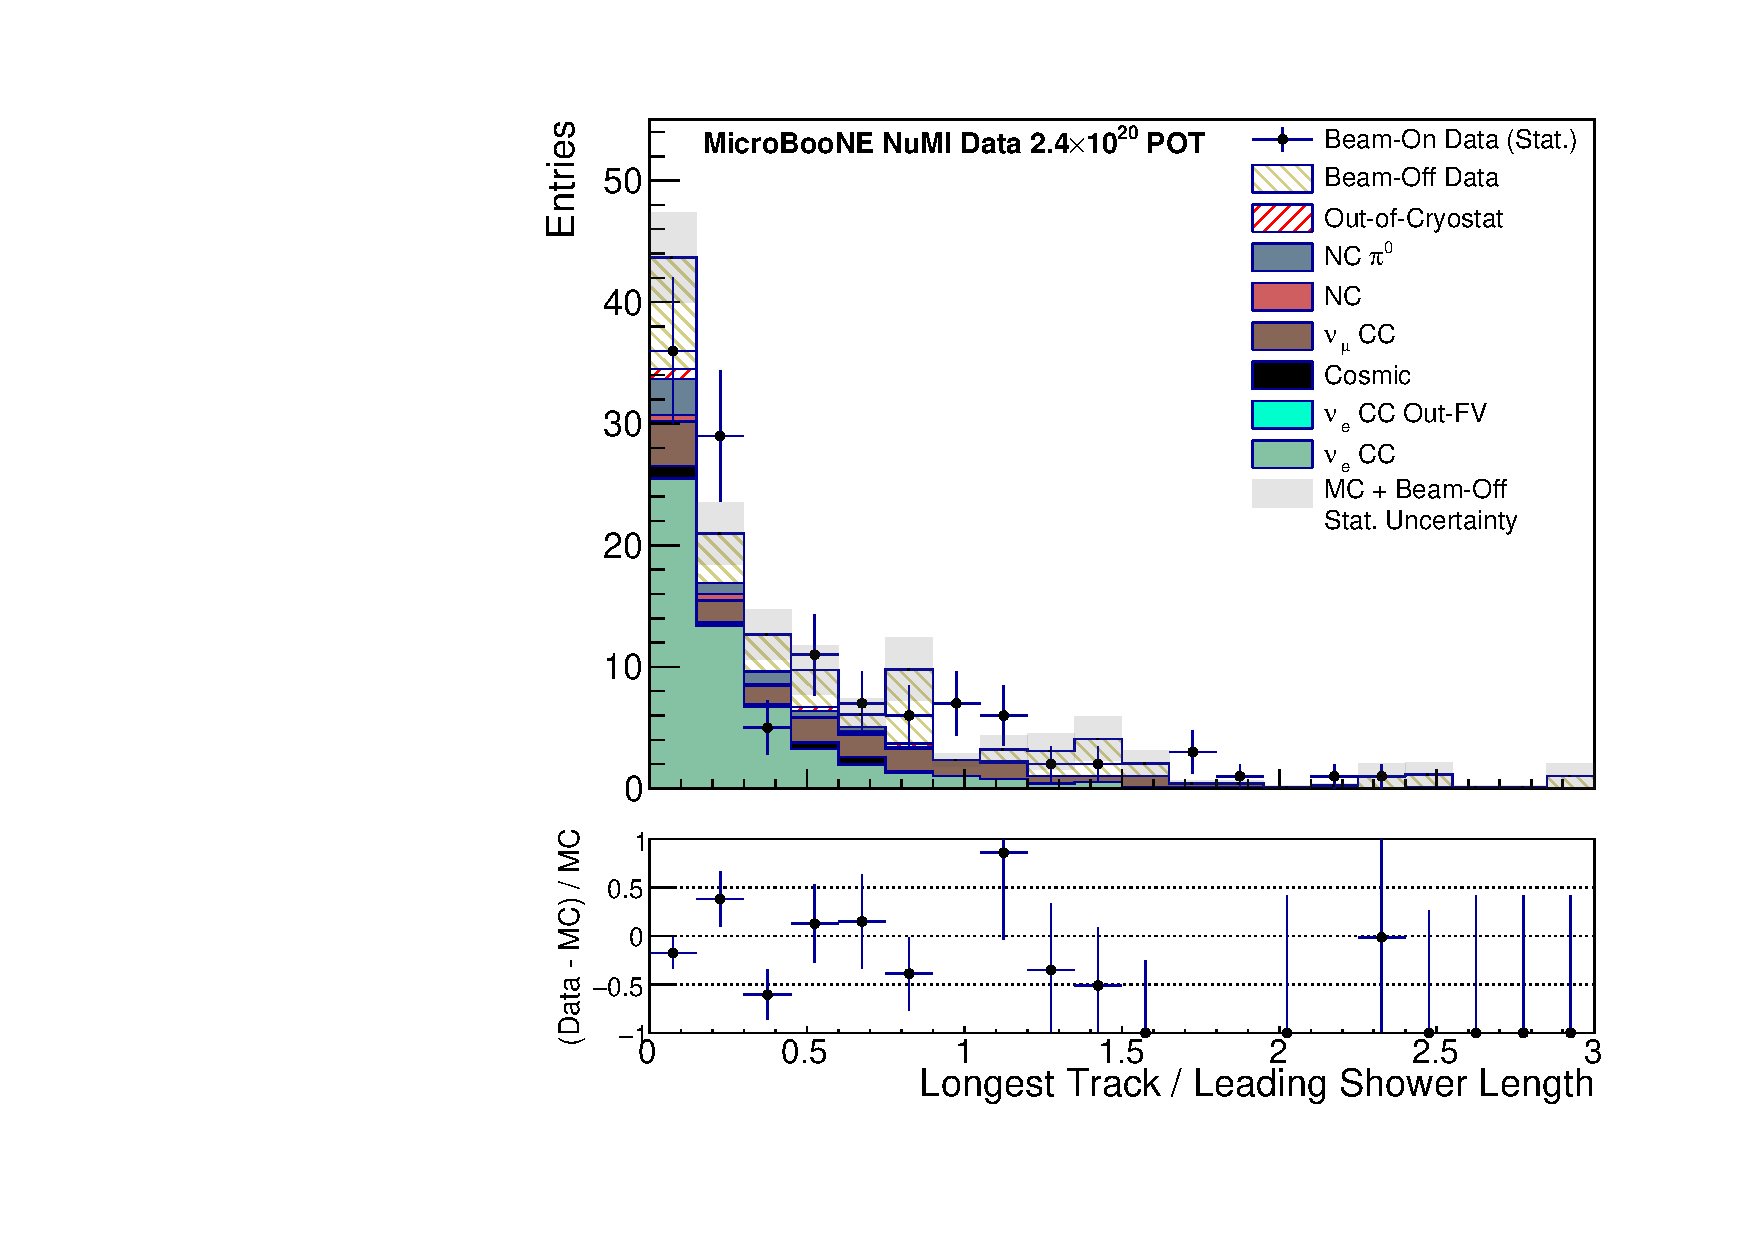
\includegraphics[width=\linewidth]{plots/post_leading_shower_trk_lengths_data.pdf}
\caption{Comparison of data (points) to the stacked prediction (MC + NuMI beam-off data) for the ratio between the longest track and the leading shower length following the selection requirement on the shower hit density. The threshold is placed at 1.0, where all neutrino candidates that have a track longer than the leading shower are removed.}\label{post_leading_shower_trk_lengths_data}
\end{figure}

To increase the purity of \textit{shower + track} topologies, we require that both the reconstructed start and end of the track are contained inside the fiducial volume. This requirement is particularly effective at rejecting long cosmic rays or muons which cross the fiducial volume and are associated to a shower inside the fiducial volume. This has a small impact on the signal selection and results roughly in a 3\% increase in purity. 

%`Overall, these final selection cuts result in about a 6\% drop in efficiency to the final selection efficiency of 9.1\%,  and an increase of about 5\% in purity, removing primarily cosmic, $\nu_{\mu}$ CC backgrounds and a small number of NC interactions, resulting in the final purity of 38.6\%.

The final number of neutrino candidates remaining after each selection stage is shown in Table \ref{cutflowtab}. 

%\begin{table*}[htbp]
%\center
%\begin{tabular}{l | c | c | c || c | c }
%Selection stage & Signal & Beam bgd. & Cosmic bgd. & Efficiency [\%] & Purity %[\%]\\
%\hline
%(1) Pre-selection & 641.26 & 3501.13 & 64703.32 & 69.4 & 0.9 \\
%(2) Flash matching & 422.17 & 1756.88 & 7660.31 & 45.7 & 4.3 \\
%(3) Vertex reconstruction quality & 334.09 & 1165.29 & 5462.75 & 36.2 & 4.8 \\
%(4) Shower hit threshold & 277.25 & 464.73 & 852.25 & 30.0 & 17.4 \\
%(5) Electron-like shower cuts & 139.59 & 97.83 & 179.53 & 15.1 & 33.5 \\
%(6) Final tuning cuts & 85.78 & 35.90 & 97.32 & 9.1 & 38.6 \\
%\hline
%\end{tabular}
%\caption{A summary of the number of signal, background and cosmic numbers (scaled to the data POT/triggers), and the efficiency and purity for different stages of the selection.\label{cutflowtab}}
%\label{cutflowtab}
%\end{table*}

\subsection{Electron-Photon Separation}\label{sec:dEdx}

A key requirement of any analysis searching for electron neutrinos is the ability to differentiate electrons originating from $\nu_e$ CC interactions from photons originating from any backgrounds. The two main features that separate interactions containing electrons from those with photons are the dE/dx at the start of the shower and the distance between the shower and the interaction vertex. The latter is only well-defined when another charged particle is present at the interaction vertex. Electron-photon separation in a LArTPC has previously been demonstrated using a semi-automated reconstruction chain \cite{Acciarri:2016sli} and only leveraging the dE/dx. 
%With the data and MC samples used in this measurement we can demonstrate the full electron-photon separation with a fully automated analysis chain in a LArTPC for the first time. 
In this measurement, we demonstrate  for the first time both of the electron-photon separation techniques that the LArTPC technology offers using a fully automated analysis chain.

To examine the performance of the electron-photon separation variables, we isolate the dE/dx and shower vertex distance selection steps on the leading shower by moving them to the end of the analysis chain; this ensures that the upstream part of the selection chain identifies neutrino interactions with a well-defined leading shower. For this study, we additionally require the leading shower $\theta$ to be between 0$^{\circ}$ and 60$^{\circ}$. This focuses on the topologies unaffected by the absence of dynamically induced charge in our simulation chain and with dE/dx best reconstructed on the collection plane wires. The very good agreement between the  data and MC samples allows us to utilize the MC sample, which provides true information about the nature of the leading shower, to determine the power of the two separation methods.

After applying the $\nu_e+\bar{\nu}_e$ CC selection without the dE/dx and shower vertex distance selection steps, we obtain a sample of 1995 simulated neutrino events. In this sample, the true particle responsible for the leading shower is an electron in 48\% of cases, a photon in 39\% of cases with 13\% remaining for other particles. We then examine the individual and combined effect of applying the dE/dx and the shower to vertex distance selection requirements on these three groups. The value of dE/dx is required to be between 1.4 and 3~MeV/cm and the distance between the shower and the vertex to be less than 4~cm apart. The combination of these two requirements selects 59\% of electron neutrino events and rejects 81\% of photon backgrounds and over 61\% of other backgrounds. When applying the requirements individually, the dE/dx is the significantly more powerful method of rejecting events with photons removing 73\% of those backgrounds by itself compared to 28\% for the shower distance to vertex. It is also responsible for the bigger drop in our efficiency to select electrons: 35\% compared to 11\%. We also investigate the effect of the shower to vertex distance selection requirement on a subset of events with at least one candidate track present. For this sample, the selection requirement has an improved performance in rejecting photon backgrounds with 47\% rejected compared to 28\% for events where we do not require the presence of a reconstructed track. The summary of the performance for each selection requirement applied individually and combined can be found in Table~\ref{tab:ele-phot}.


\begin{table}[htb]
\center
\caption{Survival rate of a sample of 1995 neutrino events where the leading shower is classified as originating from an electron, photon, or other based on MC information. The EM shower selection row refers to the $\nu_e+\bar{\nu}_e$ CC selection without the dE/dx and shower to vertex distance selection requirements. The subsequent rows show the effect of the dE/dx and shower distance to vertex selection requirements applied individually and combined for this sample of events. The final row shows the performance of the shower vertex distance selection requirement applied to events with at least one candidate track present. \label{tab:ele-phot}}
\begin{tabular}{c  c  c  c  } 
\hline
\hline
Selection stage & Electrons & Photons & Other \\
\hline
EM Shower Selection & 951 & 771 & 273  \\
dE/dx (only) & 65\%  &  27\% & 52\%  \\
Shower-Vertex Dist. (only) & 89\% & 72\% & 73\% \\
Combined & 59\% & 19\% & 39\% \\
\hline
Shower-Vertex Dist.  & 89\% & 53\% & 64\% \\
(only, $\geq$ 1 track) & & & \\
\hline
\hline
\end{tabular}
\end{table}


\begin{figure}[tbh!]
\center
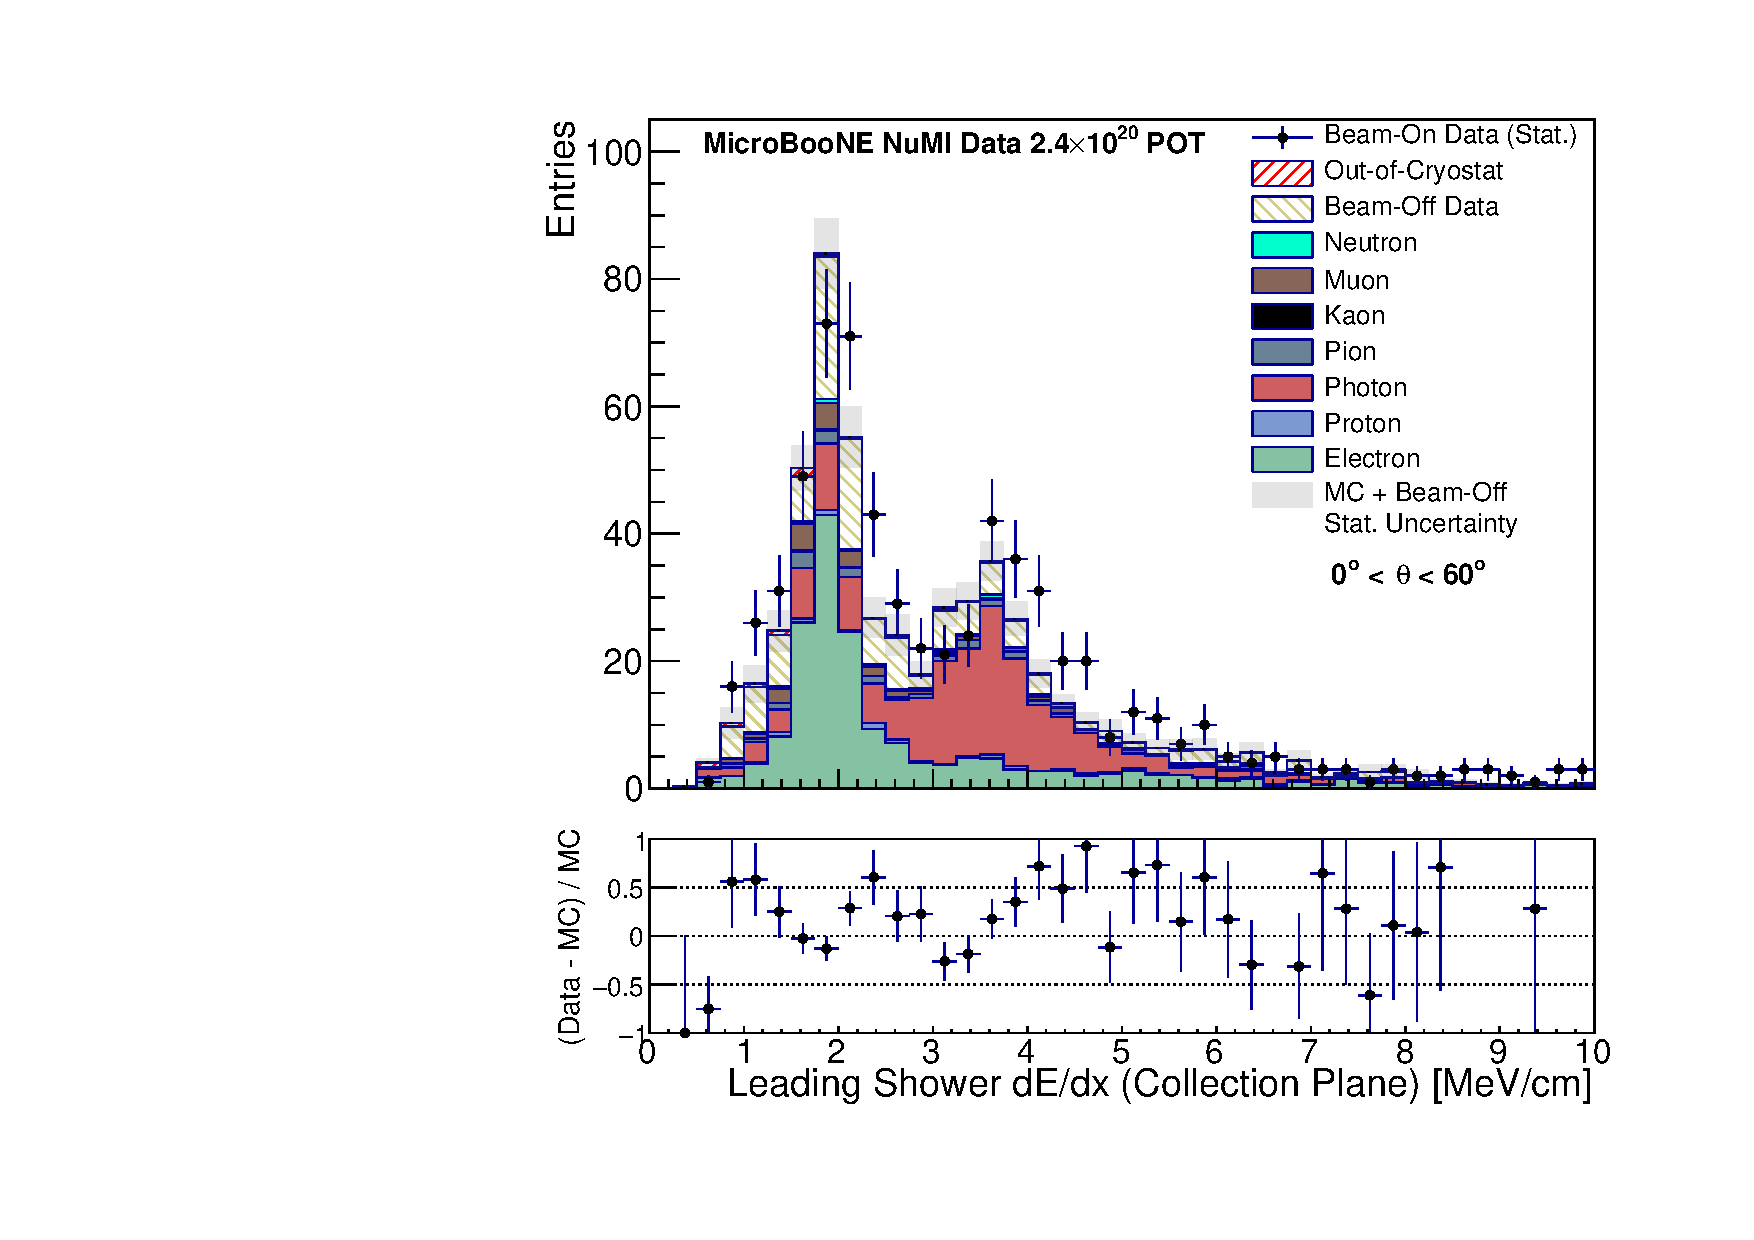
\includegraphics[width=\linewidth]{plots/post_cuts_dedx_true_particle_slice1.pdf}
\caption{dE/dx of leading showers for neutrino candidates broken down by particle type. This plot is made for leading shower $\theta$ between 0$^{\circ}$ and 60$^{\circ}$ where the reconstruction of showers is good. Electrons are gathered in the MIP peak, while most photons are around 4 MeV/cm. }
\label{post_cuts_dedx_true_particle}
\end{figure}

We find that the dE/dx variable is more effective in removing photon-induced backgrounds. Figure~\ref{post_cuts_dedx_true_particle} illustrates its separation power in rejecting the photon-like events which dominate around the 4~MeV/cm peak in the dE/dx distribution. 


%placeholder section + title for dE/dx section

\subsection{Selection Performance}

Many of the selection requirements focus on removing cosmic ray interactions reconstructed as showers. The overall decrease in the cosmic ray contamination is a factor of $10^{5}$ compared to the initial \texttt{Pandora} reconstruction stage which can have many reconstructed cosmic rays in a readout window. This ultimately brings the cosmic ray contamination to roughly the same size as the number of selected electron neutrino and antineutrino interactions. The remaining non-cosmic backgrounds contribute to approximately 19\% of the selected neutrino candidates. This demonstrates the selection's ability to reliably remove beam-induced backgrounds such as $\nu_{\mu}$ CC and $\pi^{0}$ interactions.  We find that the selection is sensitive to neutrino events where the final state electron momentum is higher than 48 MeV/c, and includes the entire angular phase space of the electron.

\begin{figure}[htb]%yes
% \center
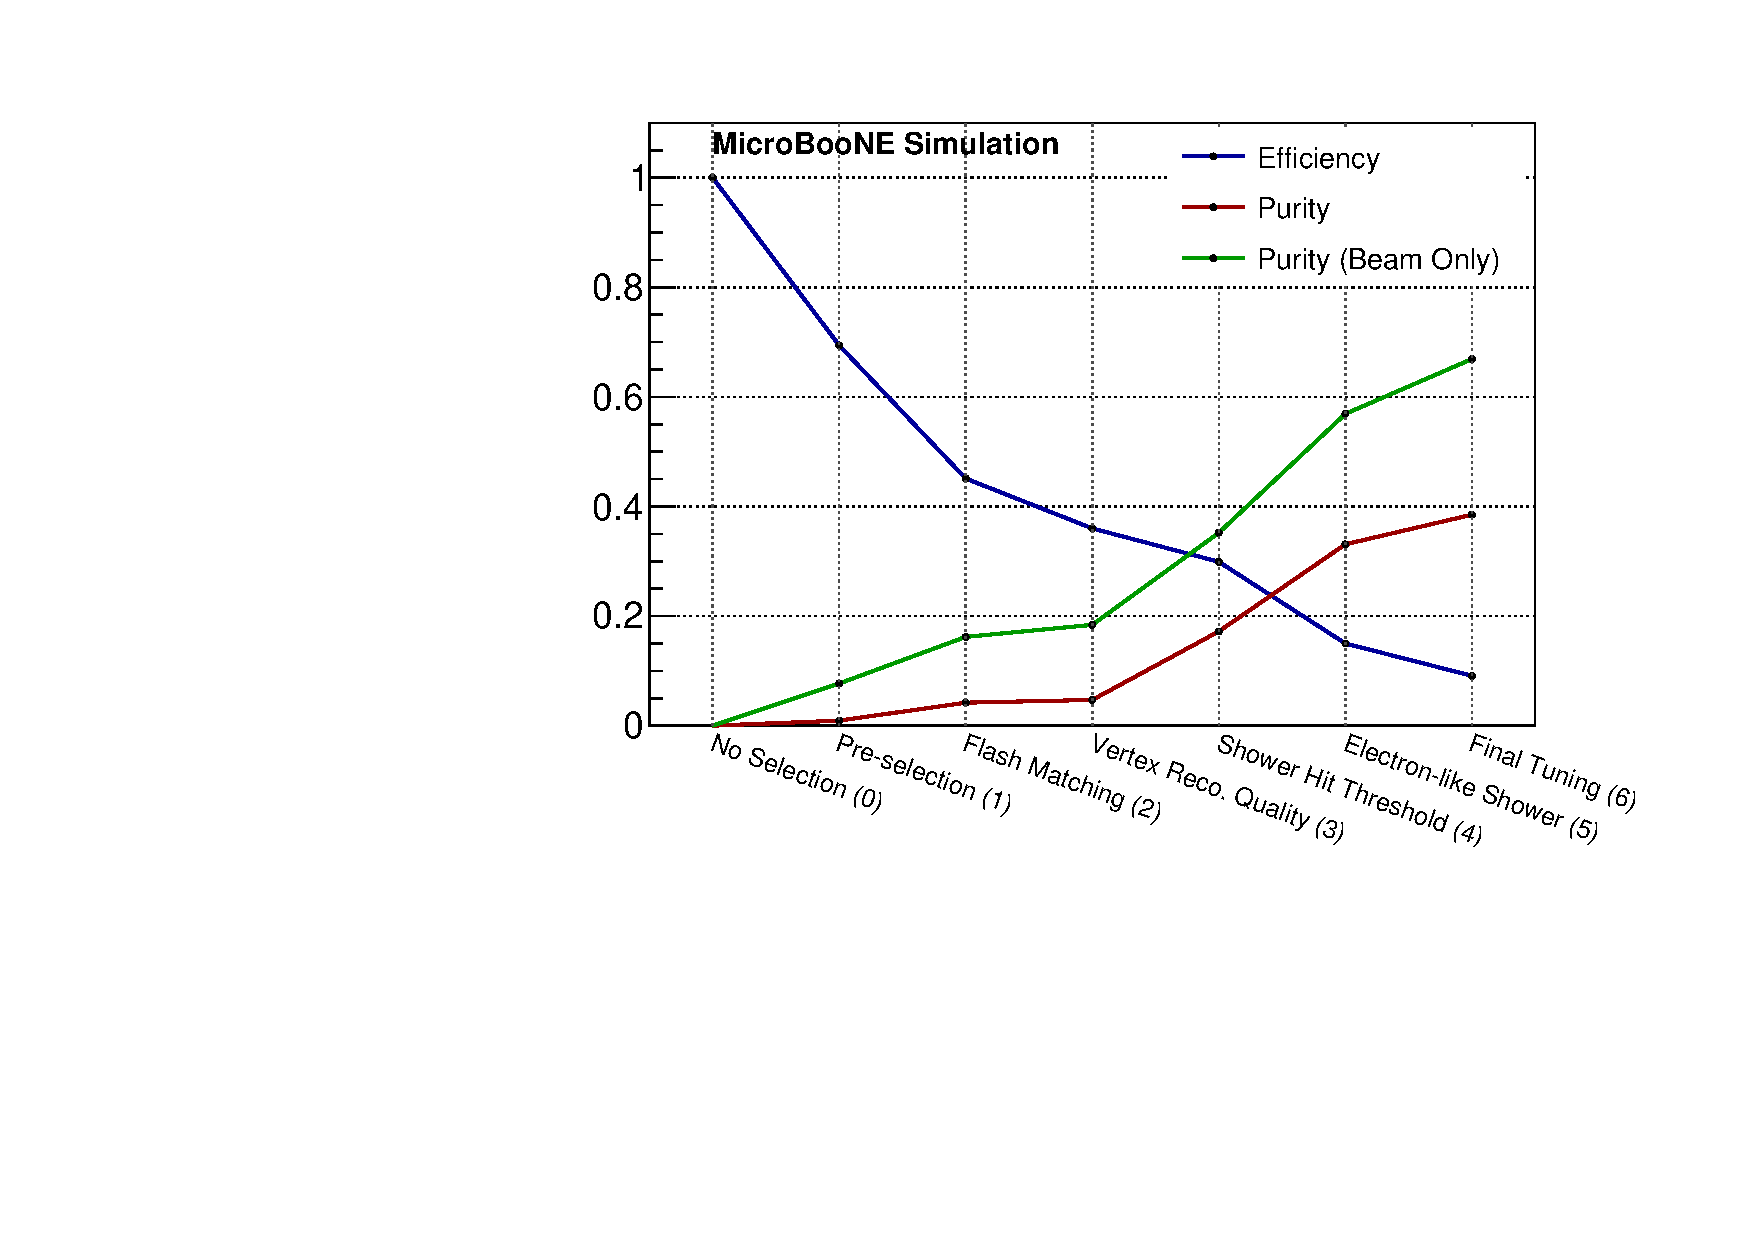
\includegraphics[width=0.49\textwidth]{plots/efficiency_plot_mcc8.pdf}
\caption{Summary of the selection performance, including efficiency, purity, and purity (beam only). The beam only purity corresponds to the selection purity if cosmic backgrounds could be completely removed.}\label{efficiency_purity}
\end{figure}

A summary of the purity and efficiency at different stages of the selection can be seen in Fig.~\ref{efficiency_purity}. The steepest decrease in the efficiency, once the basic pre-selection is applied, occurs with the application of the shower opening angle and dE/dx selection requirements which are both included in the electron-like shower category. For the latter the decrease occurs because of the difficulty in calculating the dE/dx for the shower direction of certain signal events. This is also the step with the largest increase in purity. With improvements to calculating dE/dx for all shower directions, this variable is expected to become even more powerful. The beam-only purity (in green) is shown in Fig.~\ref{efficiency_purity} and has a final value above 60\%. This is calculated by considering only beam-induced backgrounds which would be the ideal case if all cosmic ray backgrounds in this analysis could be completely removed. In future analyses with improved cosmic rejection tools such as using the cosmic ray tagger system installed around MicroBooNE, contamination from cosmic ray backgrounds should significantly decrease which will enable much higher purities and improved selection performance. The final selection efficiency is $9.1\% \pm 0.3\%$ for the $\nu_e$ + $\bar{\nu}_e$ sample, which can be divided into $8.8\% \pm 0.4\%$ and  $12.2\% \pm 1.0\%$ for $\nu_{e}$ and $\bar{\nu}_e$ respectively.
